\documentclass{article}
\usepackage{graphicx} % Required for inserting images
\usepackage{pgf}
\usepackage{lmodern}
\usepackage{import}
\usepackage{booktabs}
\usepackage{tabu}
\usepackage{float}
\usepackage[hidelinks]{hyperref}
\usepackage{amsmath}
\usepackage{amsfonts}
\usepackage[margin=1in]{geometry}
\usepackage{pythonhighlight}
\usepackage[toc]{appendix}
\usepackage{float}
\usepackage{placeins}

\setlength{\parskip}{1em}
\setlength{\parindent}{0em}

\begin{document}
\begin{titlepage}
    \begin{center}
        \vspace*{7cm}

        \Huge
        \textbf{Polarisation of Light}

        \vspace{0.5cm}
        \LARGE
        PHYS3114 - Electrodynamics

        \vspace{1.5cm}

        \textbf{Toby Nguyen - z5416116}
    \end{center}
\end{titlepage}

\tableofcontents

\section{Revised Plots}
\begin{figure} [H]
    \centering
    \scalebox{0.75}{\input{quarterwaveplate.pgf}}
    \caption{Normalised plot of intensity versus angle for a quarter 
    wave plate. The intensity is bound within 20\% of the mean which 
    displays less angular dependence than no quarter wave plate but 
    still some dependence nonetheless. }
\end{figure}
\begin{figure} [H]
    \centering
    \scalebox{0.75}{\input{quarterpolarplot.pgf}}
    \caption{Polar plot of the intensity versus angle for the quarter 
    wave plate. We notice it is jagged and not following clear 
    curvature, potentially indicating high random error in the data 
    collected.}
\end{figure}
\begin{figure} [H]
    \centering
    \scalebox{0.75}{\input{circularwaveplate.pgf}}
    \caption{Normalised plot of intensity versus angle for the circular 
    wave plate. We should expect the intensity to be independent of the 
    angle measured however experimentally we find that is not the case.}
\end{figure}
\begin{figure} [H]
    \centering
    \scalebox{0.75}{\input{circpolarplot.pgf}}
    \caption{Polar plot of the intensity versus angle for the circular 
    wave plate. We expected the polar plot to show a perfect top half of 
    a semi-circle.}
\end{figure}
\begin{figure} [H]
    \centering
    \scalebox{0.75}{\input{verticalr_s.pgf}}
    \caption{Fresnel equation experiment for vertically polarised light. 
    It is monotonically increasing as for light parallel to the plane 
    of incidence, it is unaffected by the polarisation due to reflection 
    from the dielectric.}
\end{figure}
\begin{figure} [H]
    \centering
    \scalebox{0.75}{\input{horizontalr_p.pgf}}
    \caption{Unlike vertical polarised light, horizontally polarised light
    is perpendicular to the plane of incidence and so will be affected 
    by the polarisation due to reflection on the dielectric material. The 
    polarisation will increase up until Brewster's angle when the incident 
    light is maximally polarised. Any angle past Brewster's angle, the 
    polarisation reverses but begins to decrease.}
\end{figure}

\section{Introduction}
In this report we will explore the wave nature of light through the lens of 
polarisation. Polarisation played a pivotal role in the development of our 
understanding of light. With the polarising debate between Huygens and Newtons'
differing theories of the model of light, few features of light distinguished 
the two competing theories such as interference, polarisation and diffraction. 

Focusing in on polarisation, we want to first investigate the interaction of 
an photon scattered on a molecule. Initially, quantified by Lord Rayleigh, 
we find that the intensity of scattering is dependent on the wavelength of the 
incoming light, given that the linear dimensions of the particles are much 
smaller than the wavelength. This mechanism is driven by the notion that when 
the reflector is much smaller than the wavelength, the spreading is so great 
that the reflected waves differ very little from uniform spherical waves, i.e
little interaction between reflected light, so the law of reflection ceases 
to be applicable. However as the wavelength becomes comparable in size with 
the molecule, we have Mie scattering which will scatter light independent of 
its wavelength so it produces more opaqueness or cloudiness. The Mie scattering 
effect will increase with particle size.

\begin{figure}[H]
    \centering
    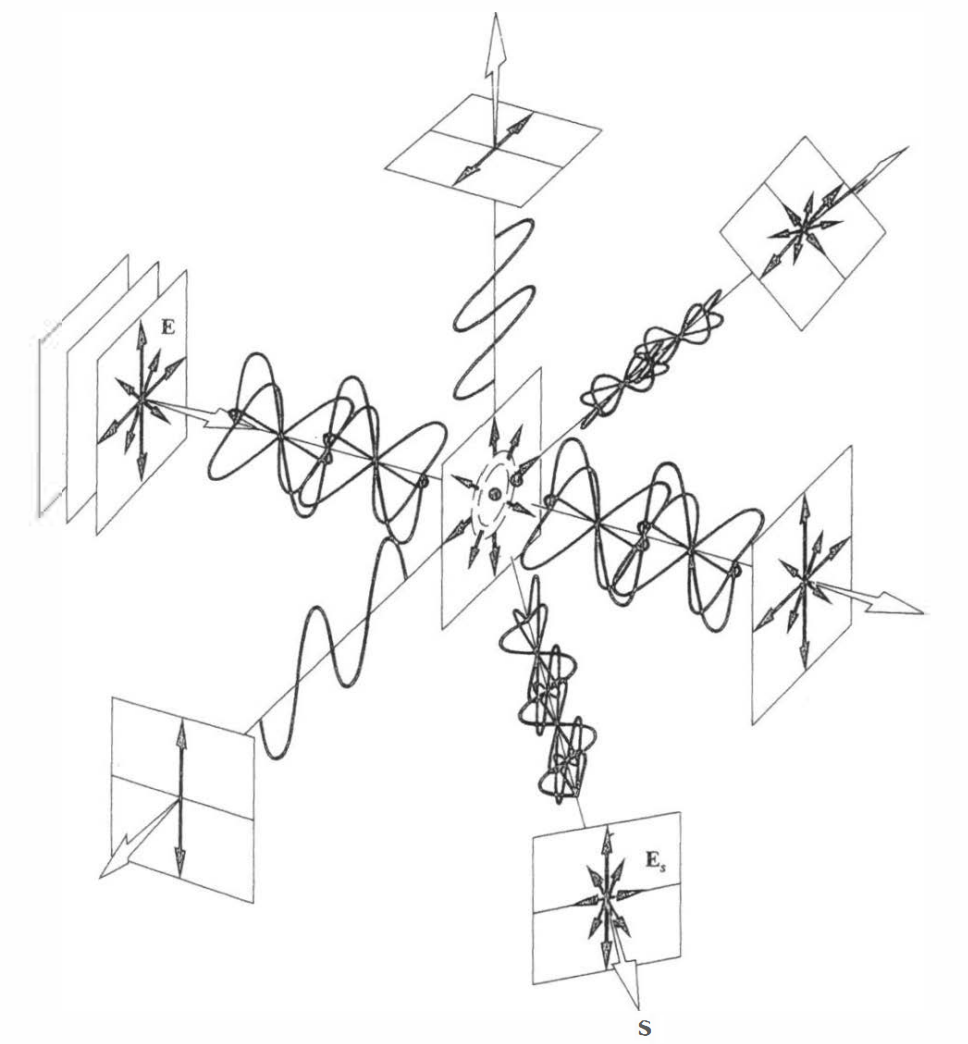
\includegraphics[width=0.5\textwidth]{scattering.png}
    \caption{Diagram showing unpolarised light incident on a molecule much 
    smaller than the wavelength of the light. Note the polarising effect of 
    scattering dependent on the angle of observation. This is due to the 
    electric dipole oscillation patterns.}
    \label{fig:scatter}
\end{figure}

When photons excite electrons such as in the case of scattering above, there 
will be energy released in the form of electric dipole radiation. The excitation 
of electrons will produce an oscillation of the dipole in the molecule. The 
electric field lines of these oscillations are shown in Figure \ref{fig:electric}
below.

\begin{figure}[H]
    \centering
    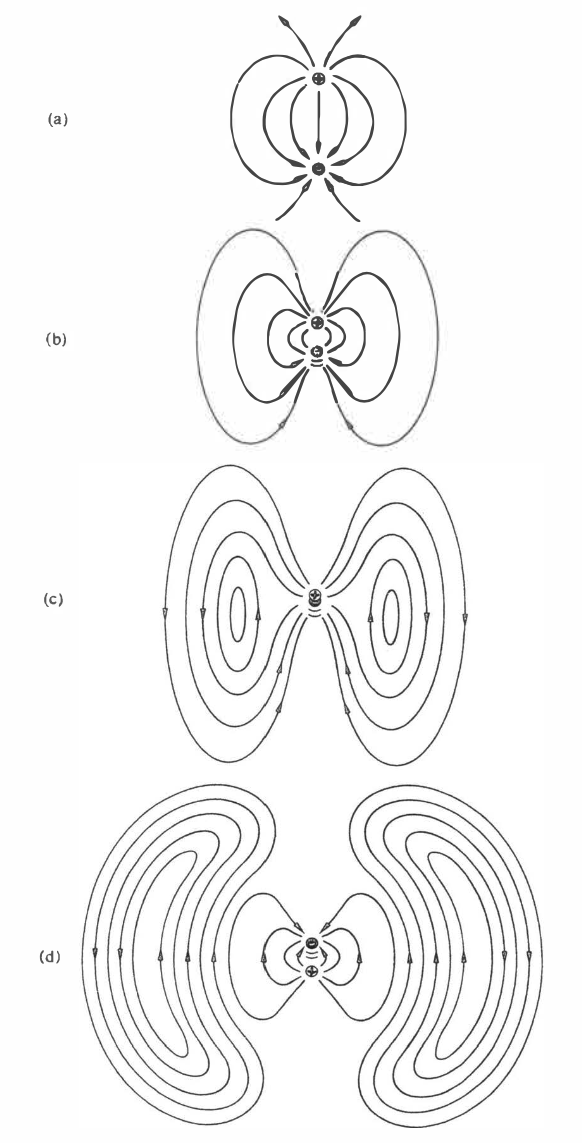
\includegraphics[width=0.5\textwidth]{efiled.png}
    \caption{Electric field lines of oscillating dipoles. Note the lack of 
    electric field in the direction parallel to the direction of oscillation.}
    \label{fig:electric}
\end{figure}

Moving away from scattering, we can further analyse the nature of polarisation 
through investigating Malus' Law. This law states that the transmitted intensity 
varies as the square of the cosine of the angle between two planes of transmission,

\begin{equation} \label{eq:malus}
    I = I_0\cos^2{\theta}.
\end{equation}

Birefringent materials are anisotropic, meaning their polarisability will depend 
on the orientation of light coming through. These materials have two axes, fast 
and slow, which possess different refractive indices. This means that there will 
be a phase delay between the two refracted beams of light whereby,

\begin{equation}
    \Delta \phi = \frac{2\pi}{\lambda}(n_e-n_o)d.
\end{equation}

If the phase delay is $\pi$, then this will lead to a rotation of linear polarisation.
Quarter-wave plates have phase delays corresponding to $\frac{\pi}{2}$. Circular 
polarisation of light can be done by taking linearly polarised light and transmitted 
it through a quarter wave plate.

The phenomenon of polarising light can also be found when light is reflected by dielectrics
materials.

\begin{figure}[H]
    \centering
    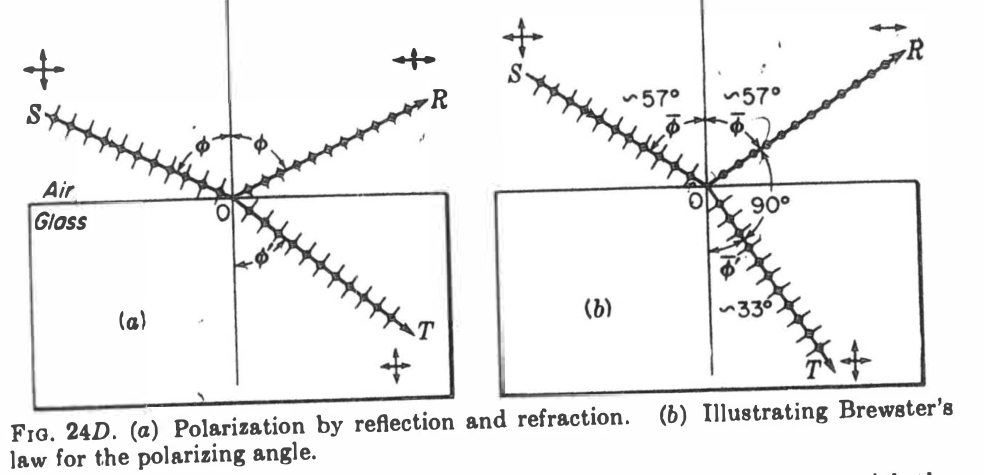
\includegraphics[scale=0.4]{brewsters.png}
    \caption{Diagram showing a special angle where the reflected beam of light becomes 
    fully polarised in one direction. This is because of the direction of the electric 
    dipole radiation mentioned before, now it is the reradiation that generates the 
    reflected beam and so only polarised light orthogonal to the plane of incidence 
    will be produced.}
    \label{fig:brewsters}
\end{figure}

Using Snell's law, we can derive the equation for Brewster's angle for incident light 
coming from air,

\begin{equation} \label{eq:brewsters}
    \tan{\theta_B} = n.
\end{equation}

At different angles, the reflected light is only partially polarised and so arises 
two orthogonal components of the light, one parallel to the plane of incidence, 
subscripted $p$ and one perpendicular to the plane of incidence, subscripted $s$. The 
reflectance coefficients describes the percentage of light reflected and can be decomposed 
into these two different alignments. Derived by Fresnel, his laws of reflection states that,

\begin{equation} \label{eq:Fresnels}
    \frac{R_s}{E_s} = \frac{\sin{(\theta - \theta')}}{\sin{(\theta + \theta')}},
\end{equation}

and

\begin{equation} \label{eq:Fresnelp}
    \frac{R_p}{E_p} = \frac{\tan{(\theta - \theta')}}{\tan{(\theta + \theta')}}.
\end{equation}

When the light hits the dielectric material at the normal incidence, we can say that 
$\theta$ and $\theta'$ become small and so we can equate the sines to the tangents, 
combining our two reflectance equations into one simple and elegant result,

\begin{equation}
    r = \frac{R^2}{E^2} = \frac{(1-n)^2}{(1+n)^2}.
\end{equation}

In the case of metals which have a complex refractive index with a imaginary coefficient 
k to denote the absorption strength of the material, we have the generalised equation,

\begin{equation} \label{eq:reflectance}
    R = \frac{(1-n)^2+k^2}{(1+n^2)+k^2}.
\end{equation}

Different angles of incidence will also influence the direction of polarisation of the 
reflected beam, hence the existence of the Brewster's angle. As Brewster's angle represents
the point at which the light is maximally polarised, this must lead to it being the point 
at which the polarisation direction of the parallel component switches.

\begin{figure}[H]
    \centering
    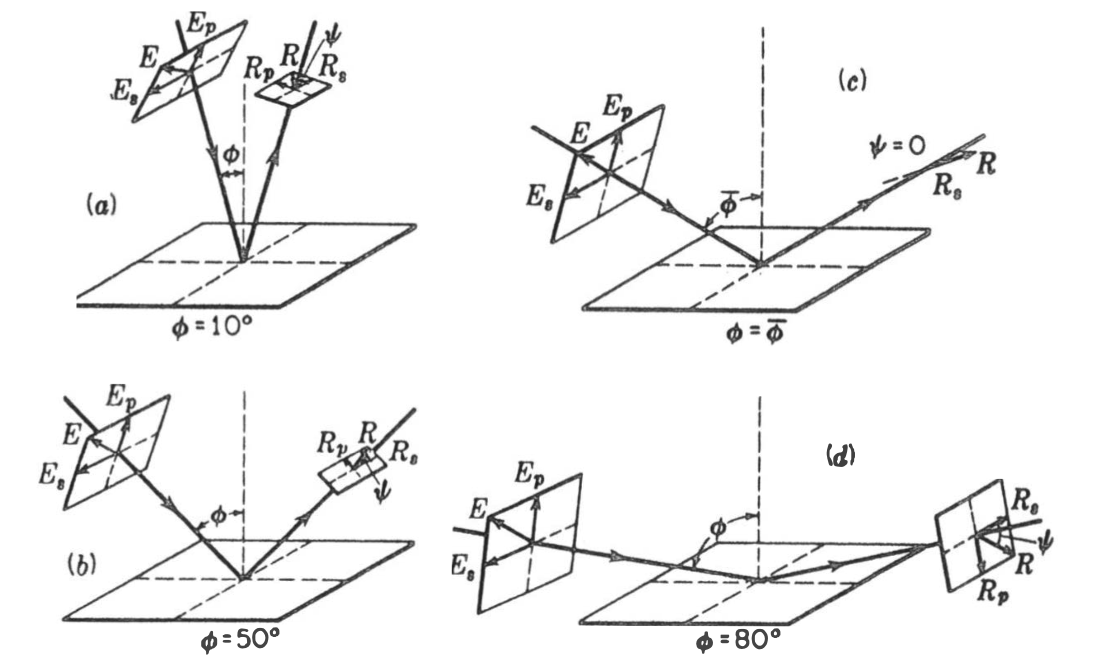
\includegraphics[width=0.5\textwidth]{polarisationofreflectedbeam.png}
    \caption{Light incident on a dielectric will produce a polarised reflected beam whose
    polarisation is dependent on the angle of incidence compared to the Brewster's angle.}
    \label{fig:reflectedbeam}
\end{figure}

Finally, light incident on a metal will be partially absorbed and reflected, depending on 
the refractive index of the metal. Aforementioned, there exists a $k$ term to represent the
metal's absorption strength and so the phase delay upon reflection is also dependent on the 
finite peneration depth of light into the material, given by,

\begin{equation} \label{eq:metalphasedelay}
    \Delta\phi = \tan^{-1}{\left(\frac{2k}{1-n^2-k^2}\right)}.
\end{equation}

\section{Jones vectors}
Throughout the report, we will be using Jones vectors and matrices to represent the tranmission 
of light. Jones vectors are representations of a polarisation state, generally denoted as,

\begin{equation}
    \textbf{J} = \begin{pmatrix}
        E_{0x} \\
        E_{0y}
    \end{pmatrix}.
\end{equation}\footnote{Phase changes will be omitted as we will only be using Jones notation
to derive relationships for intensity of light.}

Once we have a polarisation state, we can apply polarisers on it, represented by Jones matrices. 
The action of a polariser angled at $\theta$ on an input polarisation state is given by,

\begin{equation}
    \textbf{J'} = R(-\theta)PR(\theta)\textbf{J},
\end{equation}

where $R$ is the rotation matrix and $P$ is the polariser used.

The intensity of light can then be found by taking the magnitude or norm of the vector $\textbf{J'}$.

\section{Experimental Setup and Error Analysis}
The most basic setup is shown in Figure \ref{fig:diagram} below.

\begin{figure}[H]
    \centering
    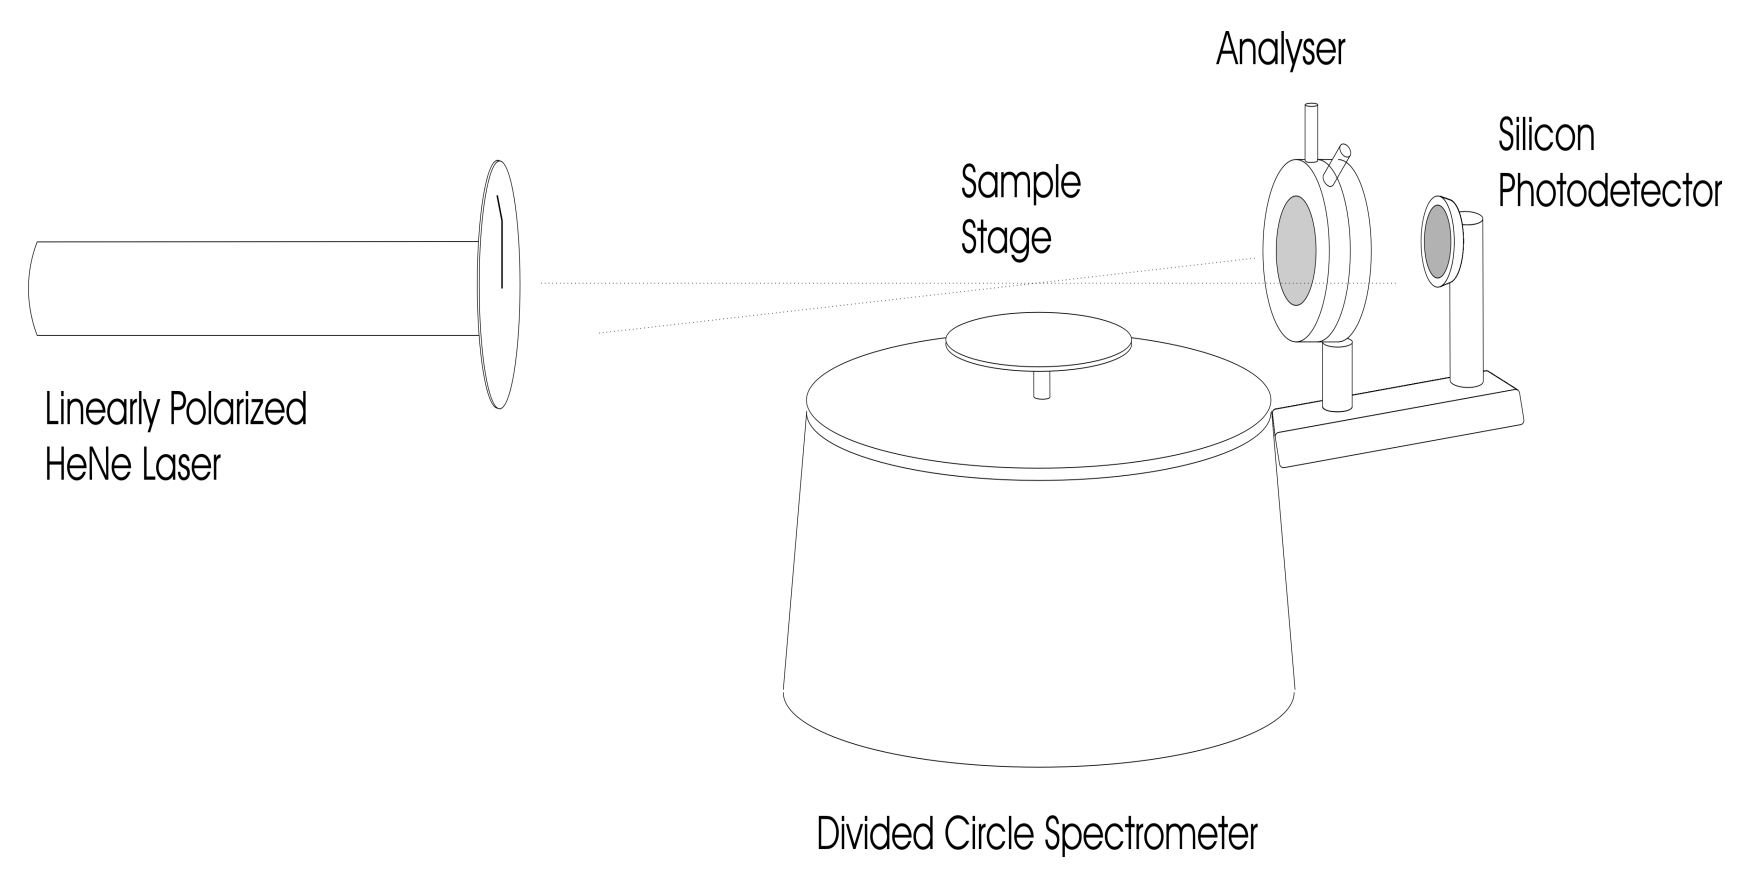
\includegraphics[width=0.8\textwidth]{experimentsetup.png}
    \caption{Schematic drawing of a basic experimental layout. Note that the spectrometer posseses 
    two measurements, one for the orientation of the Vernier table, i.e the direction of the sample
    stage with respect to the laser and the second being the spectrometer arm in relation to the 
    sample stage. The analyser and photodetector are also initially aligned with the laser in 
    parallel.}
    \label{fig:diagram}
\end{figure}

The main driver of systematic error in this experiment was the maximum precision in measuring angles. 
There were four different angle measurements, one for the polariser in front of the laser, which had 
increments of 1 degree thus an absolute error of $\pm 0.5^\circ$. This was the same for the analyser 
in front of the photodiode. The spectrometer came in increments of $\frac{1}{3}^\circ$, indicating an 
absolute error of $\pm\frac{1}{6}^\circ$ however due to wear and visibility, the absolute error was 
adjust to be $\pm0.25^\circ$. The spectrometer was used to measure the orientation of the Vernier table 
as well as the spectrometer arm. The uncertainty in the laser and the photodetector was taken to be 
negligible. The next major source of systematic error would be the misalignment of the components in 
the experiment. This would lead to unintended reflected beams from various components which would 
potentially alter the intensity reading by the photodetector. We quantified this error to be $1\%$.
The error analysis for each experiment can be found in the Python code below.

\begin{python}
#Error analysis

#Error for Experiment 1
#Sources of Error: Alignment of setup (1%) + Reading of halfwave plate (+- 0.5 / 199) + Reading of Spectrometer arm (+-0.25/90) + Analyser readings from 0 to 180

x0 = np.linspace(10,180,18)
analyser_error_exp1 = [0.5/i for i in x0]
rms_analyser_exp1 = np.sqrt(np.mean(np.square(analyser_error_exp1)))

exp1_err = np.sqrt(0.01**2+(0.5/199)**2+(0.25/90)**2+rms_analyser_exp1**2)

#Error for Experiment 2
#Sources of Error: Alignment of setup (1%) + Reading of halfwave plate (+- 0.5/199) + Analyser readings from 0 to 90

x1 = np.linspace(10,90,9)
analyser_error_exp2n3 = [0.5/i for i in x1]
rms_analyser_exp2n3 = np.sqrt(np.mean(np.square(analyser_error_exp2n3)))

exp2n3_err = np.sqrt(0.01**2 + (0.5/199)**2+rms_analyser_exp2n3**2)

#Error for Experiment 4a
#Sources of Error: Alignment of setup (1%) + Table reading (0.25/330) + Table reading 2 (0.25/21) + half wave plate reading (0.5/334)
 
exp4brewsters_err = np.sqrt(0.01**2+(0.25/330)**2+(0.25/21)**2+(0.5/334)**2)

#Error for Experiment 4b
#Sources for Error: Table reading (0.25/21.66) + Intensity (0.05/75.4) + Background reading (0.05/7.9) + Table reading 2 (0.25/226) + Arm (0.25/306) + Table rotation from 0 to 30 degrees

x2 = np.linspace(5,30,6)
table_error_exp4 = [0.25/i for i in x2]
rms_table_exp4 = np.sqrt(np.mean(np.square(table_error_exp4)))

exp4bv_error = np.sqrt((0.25/21.66)**2+(0.05/75.4)**2+(0.05/7.9)**2+(0.25/226)**2+(0.25/306)**2+rms_table_exp4**2)
exp4bh_error = np.sqrt((0.25/21.66)**2+(0.05/55.3)**2+(0.05/4.4)**2+(0.25/227)**2+(0.25/306)**2+rms_table_exp4**2)

#Error for Experiment 4c
#Sources of Error: Alignment of setup (1%) + Table reading error (+-0.25/20) + Halfwave plate (0.5/221.5) + 1 Analyser Reading (0.5/312) or (0.5/236)
exp4_20_error = np.sqrt(0.01**2+(0.25/20)**2+(0.5/221.5)**2+(0.5/312)**2)
exp4_80_error = np.sqrt(0.01**2+(0.25/20)**2+(0.5/221.5)**2+(0.5/236)**2)

#Error for Experiment 5
#Sources of error: Waveplate reading (0.5/221.5) + Analyser reading (0.5/235) or (0.5/315) + Table reading (0.5/22.66) or (0.5/14)
exp5_20_error = np.sqrt((0.5/221.5)**2+(0.5/235)**2+(0.5/22.6)**2+rms_analyser_exp1**2)
exp5_79_error = np.sqrt((0.5/221.5)**2+(0.5/315)**2+(0.5/14)**2+rms_analyser_exp1**2)
\end{python}

As seen above, to account for multiple angle measurement uncertainties, the root mean squared was used 
rather than the mean. This is because higher uncertainty percentages, i.e smaller angles should be 
weighted greater.

\section{Part I}
\subsection{Method}
\subsubsection{Scattering}
In this half of the report, the setup shown in Figure \ref{fig:diagram} was used. We wanted to first 
investigate the polarisation pattern found in Figure \ref{fig:scatter}. To do so, a container of 
Dettol solution was placed onto the sample stage with a vertically polarised laser pointing directly 
into its centre, illuminating the inside and scattering red light spherically from the container. 
The analyser was then rotated to give a maximum intensity reading and the spectrometer arm was rotated
from $0^\circ$ to $90^\circ$ with respect to the beam. We should expect the intensity to remain 
constant because the incident light will excite the molecules to oscillate in the vertical direction,
maximally polarising light vertically. This was then repeated for a horizontally polarised laser 
and now we should expect intensity to decrease as we approach the perpendicular observation direction.

We want to investigate the relationship between the spatial dimensions of the scattering medium and 
the intensity of the scattering. For this, we will compare the intensity of light perpendicular to the 
beam as it passes through a solution. As we are measuring the intensity from the perpendicular observation 
point, the orientation of the polarised laser must be in the vertical direction. We compare two solutions, 
Ajax and Dettol. By eye, Dettol is a much more cloudy and opaque liquid, indicating larger molecules as 
well as a greater number of molecules. We expect the intensity of scattering then to be greater for the Ajax 
solution as the size of the molecules will be finer, allowing for a higher fraction of independent scattered 
spherical waves sourced from each incident interaction of laser to molecule.

Next, we will explore Malus' law. 

\subsubsection{Polarisation}
The initial polarisation on the laser is vertically orientated 
so we can represent this using the Jones vector,

\begin{equation}
    \textbf{y} = \begin{pmatrix}
        0 \\
        1
    \end{pmatrix}.
\end{equation}

Or more specifically,

\begin{equation} \label{eq:J}
    \textbf{J} =\begin{pmatrix}
        0 \\
        E_{oy}
    \end{pmatrix}.
\end{equation}

To find the Jones' matrix representation of an analyser at some angle 
$\theta$ to the plane of polarisation of the incoming light, we first 
consider some arbitrary reference frame for which the polariser is 
aligned with, at an angle $\theta$. So we have to introduce a rotation
matrix with angle $\theta$ to transform the coordinates into the reference 
frame of the polariser,

\begin{equation}
    \textbf{$R_+$} = \begin{pmatrix}
        \cos{\theta} & \sin{\theta} \\
        -\sin{\theta} & \cos{\theta}
    \end{pmatrix}.
\end{equation}

We can now just apply the follow Jones matrix to remove any orthogonal 
components,

\begin{equation}
    \textbf{$P_y$} = \begin{pmatrix}
        0 & 0 \\
        0 & 1
    \end{pmatrix}.
\end{equation}

Now we can transform the coordinates back into the reference frame of 
the lab by applying the rotation matrix again but with $-\theta$,

\begin{equation}
    \textbf{$R_-$} = \begin{pmatrix}
        \cos{-\theta} & -\sin{\theta} \\
        \sin{\theta} & \cos{\theta}
    \end{pmatrix}.
\end{equation}

Putting all of this together,

\begin{equation}
    \textbf{J'} = R_- P_y R_+ \textbf{J}.
\end{equation}

Computing the matrix multiplication will result in,

\begin{equation}
    \textbf{J'} = \begin{pmatrix}
        \sin^2{\theta} & -\cos{\theta}\sin{\theta} \\
        -\cos{\theta}\sin{\theta} & \cos^2{\theta}
    \end{pmatrix} \textbf{J}.
\end{equation}

Substituting in Equation \ref{eq:J}, we find,
\begin{align}
    \textbf{J'} &= \begin{pmatrix}
        \sin^2{\theta} & -\cos{\theta}\sin{\theta} \\
        -\cos{\theta}\sin{\theta} & \cos^2{\theta}^2
    \end{pmatrix} 
    \begin{pmatrix}
        0 \\
        E_{0y}
    \end{pmatrix} \\
    &= E_{0y}\begin{pmatrix}
        \cos{\theta}\sin{\theta} \\
        \cos^2{\theta}
    \end{pmatrix}
\end{align}

Taking the magnitude of the Jones vector to represent its magnitude,

\begin{equation}
    I = |\textbf{J'}|^2 = E_{0y}(\sin^2{\theta}\cos^2{\theta}+\cos^4{\theta}).
\end{equation}

Simplifying the equation and then replacing $E_{0y}$ with $I_0$,

\begin{align}
    I &= I_0(\cos^2{\theta}(1-\cos^2{\theta})+\cos^4{\theta}) \\
    &= I_0\cos^2{\theta}.
\end{align}

A result that is a little too long to display here but will be referenced in 
the appendix, in Appendix \ref{eq:derivation}, is the fact that quarter wave 
polarisers will not affect the amplitude of the incoming wave, instead only 
introduce a phase delay. This means that we expect Malus's law to hold even 
for circularly polarised light, except with a phase delay.

Experimentally, to test the polarisation of light by analyser angles, quarter
wave plates and circular polarisers, we can just use the same setup as found in 
Figure \ref{fig:diagram} with the filter or no filter on the sample stage. 
The intensity versus angle plot can be created by rotating the analyser through 
180 degrees to see any periodic changes in the intensity of the transmitted 
light.

\subsection{Results}

\subsubsection{Scattering}
\begin{figure} [H]
    \centering
    \scalebox{0.5}{\input{horizontaldettol.pgf}}
    \hspace{0.5cm}
    \scalebox{0.5}{\input{verticaldettol.pgf}}
    \caption{Graphs of intensity of scattering versus azimuthal angle
    from $0^\circ$ to $90^\circ$. (a) Horizontal polarised light 
    (b) Vertical polarised light.}
    \label{plot:dettol}
\end{figure}


\begin{figure} [H]
    \centering
    \scalebox{0.75}{\input{experiment1.pgf}}
    \caption{Curves describing intensity of scattering at a 
    perpendicular observation angle to the beam as a function of 
    the angle of the analyser for Ajax and Dettol superimposed on the 
    same plot with different y axes. The important thing to note is the
    fact that they are in phase but with different amplitudes.}
    \label{plot:ajaxdettol}
\end{figure}

\subsubsection{Polarisation}

\begin{figure} [H]
    \centering
    \scalebox{0.5}{\input{maluslawstraightline.pgf}}
    \hspace{0.5cm}
    \scalebox{0.5}{\input{maluslaw.pgf}}
    \caption{Results from Malus law experiment. (a) Intensity versus 
    $\cos^2{\theta}$ (b) Intensity versus angle of the analyser.}
    \label{plot:malus}
\end{figure}

\begin{figure} [H]
    \centering
    \scalebox{0.5}{\input{quarterwaveplate.pgf}}
    \hspace{0.5cm}
    \scalebox{0.5}{\input{circularwaveplate.pgf}}
    \caption{Similar plots to the Malus' law experiments. (a) Quarter
    wave plate (b) Circular polariser. Note the phase shift between 
    the two curves.}
    \label{plot:quartercirc}
\end{figure}

\subsection{Analysis}
Our scattering results strongly reflect the theoretical model proposed 
in Figure \ref{fig:scatter}. We found that for the intensity of 
scattered of light as a function of azimuthal angle, $\phi$, or rotation 
of the spectrometer arm, it decrease monotonically from $0^\circ$ to 
$90^\circ$ in the case of horizontally polarised incident light. It 
seemed to decrease linearly past $20^\circ$ but we currently don't have 
a model we can fit this to explain this relationship so we can only 
observe from a quasi-quantitative manner. Similarly, we found that 
when the incident light was vertically polarised, the intensity of the 
scattering along the azimuthal was largely constant, with some minor 
flunctuations due to deviations in background noise. Nevertheless, this 
agrees with our theoretical model.

We also found that the size of the molecules that scatter the photons 
influences the angle of scattering as postulated by Mie scattering. 
This is shown as the intensity of scattering at the perpendicular 
observation angle is much weaker for Ajax than Dettol because Dettol 
molecules are much bigger. However, we find that the polarisation of 
the scattered light is the same irregardless of molecule size as we 
can see the phase of the two curves are equal.

We find in Figure \ref{plot:malus}, the experimental data matches with 
a best fitting cosine squared function without any error.

A circular polariser is comprised of a linear polarised in front of
a quarter wave plate. We find that in Figure \ref{plot:quartercirc}(a),
the coefficients of the best fitting cosine squared function is given 
in the legend. Comparing this with the coefficients found in Figure
\ref{plot:quartercirc}(b), we can see that the amplitudes differ by 
a factor of 2 but more importantly the phase difference is $215.92
^\circ$. We expect the amplitude to be halved as placing a linear 
polariser in front of the quarter wave plate will half the effectively
unpolarised light (as we don't know the orientation of this linear 
polariser). The phase shift is purely due to the quarter wave plate 
although this value heavily differs with the expected value of $90^\circ$. 
A better way to find the phase shift is to locate the angle 
of the minimums and subtract them. This method yields a result of 
$50.2^\circ$. However we have to consider that this is in cosine 
squared space where the wavelength is halved so this result will 
translate to a final phase delay of $100.4^\circ$, representing a 
$12\%$ error.

We can verify the composition of the circular polariser but taking 
the ratios of each side facing the laser. We found this ratio from 
Side 2 to Side 1 to be $15540/0.524 \approx 30 000$, i.e the side 
with the linear polariser must face the laser first for the light 
to be properly polarised before being 'twisted'. 

\section{Part II}
\subsection{Method}
In the latter half of the report we want to explore the polarisation 
of light caused by reflecting on different materials, namely a 
dielectric and a metal.

\subsubsection{Dielectrics}
In dielectric materials such as glass, there exists a special angle,
denoted as the Brewster's angle for which the reflected beam of light 
is maximally polarised and the angle between the reflected beam and 
the refracted beam is 90 degrees. We want to find this angle so we can 
accurately calculate the refractive index of the glass prism to then 
confirm Fresnel's equations.

To find Brewster's angle we replace the photodetector with a white 
screen and then remove the analyser attached to the spectrometer arm.
The prism is then placed on the sample stage with the vertically 
polarised laser incident at its normal. We then rotate the polarisation 
of the laser until the reflected beam on the white screen hits a 
minimum, this happens because the incoming polarised light is now 
perpendicular to the plane of incidence, causing further partial 
polarisation of the reflected beam. Once, at the minimum, the table is 
incrementally rotated and the process is repeated until we achieve the 
absolute minimum and the angle of incidence is defined as Brewster's 
angle.

Since we have the refractive index, we want to verify Fresnel's equations.
At the normal incidence, the associated Jones matrix to find the reflected 
beam is 

\begin{equation}
    \textbf{M} = \begin{pmatrix}
        r & 0 \\
        0 & r
    \end{pmatrix}.
\end{equation}

Derived in Appendix \ref{eq:derivation2}, we find that the intensity of 
the reflected ray divided by the intensity emitted is directly equal to 
the reflectance coefficient. There are many ways of obtaining this 
reflectance coefficient at the normal incidence. We can do a direct 
measurement by taking the intensity of the reflectance and dividing it 
by the measured intensity of the laser beam. We can also use Fresnel's 
equation \ref{eq:reflectance} where k is 0 in this case. We will compare 
these values with the fitted value found experimentally.

\subsubsection{Metals}
Finally we want to determine the optical constants of the aluminium 
mirror. To do this we need to solve Equations \ref{eq:reflectance} and 
\ref{eq:metalphasedelay} simutaneously as there are two unknowns. We 
can take two intensity versus analyser angle curves at different angle 
of incidences. Similar to experiments 2 and 3 where we just rotated 
the analyser through 180 degrees to obtain a Malus law curve, this time 
we want to produce the curves for the reflected beams for angle of 
incidences, $20^\circ$ and $79^\circ$.

\subsection{Results}
\subsubsection{Dielectrics}

\begin{figure} [H]
    \centering
    \scalebox{0.5}{\input{horizontalr_p.pgf}}
    \hspace{0.5cm}
    \scalebox{0.5}{\input{verticalr_s.pgf}}
    \caption{Minimum intensity versus azimuthal angle (a) Horizontal 
    polarisation of incident light, resulting in $R_p$. (b) Vertical 
    polarisation of incident light, resulting in $R_s$.}
    \label{plot:fresnel}
\end{figure}

\subsubsection{Metals}

\begin{figure} [H]
    \centering
    \scalebox{0.5}{\input{metal20.pgf}}
    \hspace{0.5cm}
    \scalebox{0.5}{\input{metal79.pgf}}
    \caption{Intensity versus angle of analyser plot. (a) At $20^\circ$
    to the normal. (b) At $79^\circ$ to the normal.}
    \label{plot:metals}
\end{figure}

\subsection{Analysis}
We determined Brewster's angle to be $51 \pm 0.8^\circ$. Glass is 
usually approximated to have a Brewster's angle of $56^\circ$, 
representing a $9\%$ error. Nevertheless, this translates to a 
refractive index of 1.55 for our glass prism. 

Using this value, 
we can find the reflectance coefficient using Equation \ref{eq:reflectance},
again where k is zero. This gives us an $r$ value of 0.305, representing 
roughly $31\%$ of light is reflected and so $69\%$ of light is 
transmitted. Experimentally, we found the reflectance intensity 
to be $55.3nA$ whilst the laser without any reflection was found to be 
$339nA$, giving us a coefficient value of 0.163. This represents as 
a $46\%$ deviation from the expected value given by Fresnel's equation.
We can see qualitatively in Figure \ref{plot:fresnel} that the 
experimental data deviates quite a bit away from the best fit curve 
whilst the error bars are quite low.

We also found that the angle of incidence on the glass prism will 
change the polarisation of the reflected light. Taking a measurement 
at $20^\circ$ to the normal yielded a maximal polarisation in the 
direction $312^\circ$ with respect to the analyser. Meanwhile, 
taking the same measurement but at $80^\circ$, we find that this 
angle has fallen to $236^\circ$. This was expected as the two angles 
of incidences lie on opposite sides of the Brewster angle.

Finally for the light incident on metals, we can use simutaneous 
equations to solve for n and k. From Figure \ref{plot:metals}, the 
phase difference is $12.37^\circ$. Converting this into radians,
gives us 0.216. Since we didn't obtain a reflectance measurement due 
to negligance, we have to assume a $r=0.65$. Solving the two equations
yields us $n=0.108$ and $k = 0.0727$

\subsection{Discussion}
The hardest proponent of this experiment was the alignment of the 
components. No matter how many tries it took to move each component 
around, it was difficult to align the laser directly at the detector 
without any reflected beams and then aligning the analyser to perfectly 
slide between the laser and the detector. Eventually due to the nature 
of the experiment exploring the relationship between quantities rather 
than aiming to measure a specific accurate value, perfect alignment was 
forgone.

The latter half of the experiment provided great challenges in utilising
the prism due to its shape. It was difficult to produce great 
angles of incidence to the normal so we had to forgo perfect alignment 
in order to compensate for the prism's shape.

Another large issue was the lack proper uncertainty analysis when it 
comes to angles. Since the size of the angle did not matter, it was 
the size of the angle relative to other readings that did, it was hard
to quantify this value as a percentage error.

\subsection{Conclusion}
These experiments were completed in a satisfactory manner. They explored
various features and causations of polarisations however lacked the 
accuracy and precision required to draw out definitive conclusions about 
the relationships involved.

\section{Appendix}
\subsection{Pre-Work Theoretical Questions}
\subsubsection{Question 2a}
\textbf{What is the condition for linearly polarised light to 
remain unaltered as it passes through a crystal?}

For the linearly polarised light to remain unaltered, the light 
incidence needs to experience no relative phase changes. Crystals
can either be isotropic or anisotropic. In the case of isotropic 
crystals, the linearly polarised light has to be pass through the 
crystal along its polarisation axis. Anisotropic materials have a 
property known as birefringence, where the crystal has a different
refractive index for each polarisation and propagation of light. 
The linearly polarised light must enter the crystal along the 
optical axis. This means that the light will only experience the
refractive index of ordinary rays. If light were to enter the crystal
in any other direction, then it would experience two refractive indexes
which will alter the polarisation of the wave. Similarly, in biaxial
crystals, there are two optical axes (binormals) that allow light to
travel through without birefringence.

\subsubsection{Question 2b}
\textbf{What are the conditions to create circularly polarised light?}

You can use a linear polariser to get linearly polarised light first
and then use a quarter wave layer to create a circular polariser. The 
corresponding phase difference needs to be 90 degrees. To achieve this,
the formula for phase difference in uniaxial crystals can be used,

\begin{equation}
    \Delta \phi = \frac{2\pi}{\lambda}(n_e-n_o)d.
\end{equation}
By adjusting the thickness, d, of the crystal appropriately as $n_e$ 
and $n_o$ are fixed, we can obtain a phase difference of 90 degrees. 
Then the quarter wave plate needs to placed at an angle of 45 degrees
with the plane of the incident polarised light.

\subsubsection{Question 2c}
\textbf{What is the effect of a quarter wave plate on circularly polarised light?}

The quarter wave plate will introduce a 90 degree phase shift which 
will convert circularly polarised light back to linearly polarised.

\subsubsection{Question 2d}
\textbf{What is the effect of a half wave plate on circularly polarised light?}

A half wave plate will introduce a phase difference of 180 degrees, 
meaning that the handedness of the circular polarisation will switch i.e 
right handed circular polarisation will turn into left handed circular
polarisation and vice versa.

\subsubsection{Question 2e}
\textbf{Sometimes the scattering of light off particles may lead to polarisation.
Explaining in terms of scattering, why is the sky blue and why clouds are grey?}

In 1871, Rayleigh discovered that when light is scattered by molecules or 
particles much smaller than the wavelength of the light, the intensity 
of the scattered light has the following property,

\begin{equation}
    I \propto \frac{1}{\lambda^4}.
\end{equation}

This is why the sky is blue as the lower wavelengths of light, i.e bluer, are 
scattered much more. At sunset, when the sun is low of the horizon, the blue
and violet light is scattered out of the direct line of sight, giving the sky
its redder tinge. In clouds, the particles are no longer small enough for 
Rayleigh scattering and instead we look at Mie scattering. Here we find that 
the droplets of water will scatter all wavelengths equally and so clouds are
perceived as white. As the clouds become thicker, more light is absorbed and 
less sunlight can penetrate, dimming the sky and the appearance of the cloud.

When light strikes a particle, it will induce an oscillation in the charges 
of the particle, causing it to re-emit light but they do so more strongly in
directions where the electric field is perpendicular to the direction of 
observation. For the original incoming light, it becomes polarised as the 
electric field in the direction of scattering is minimised.

\subsubsection{Question 2f}

\begin{figure}[H]
    \centering
    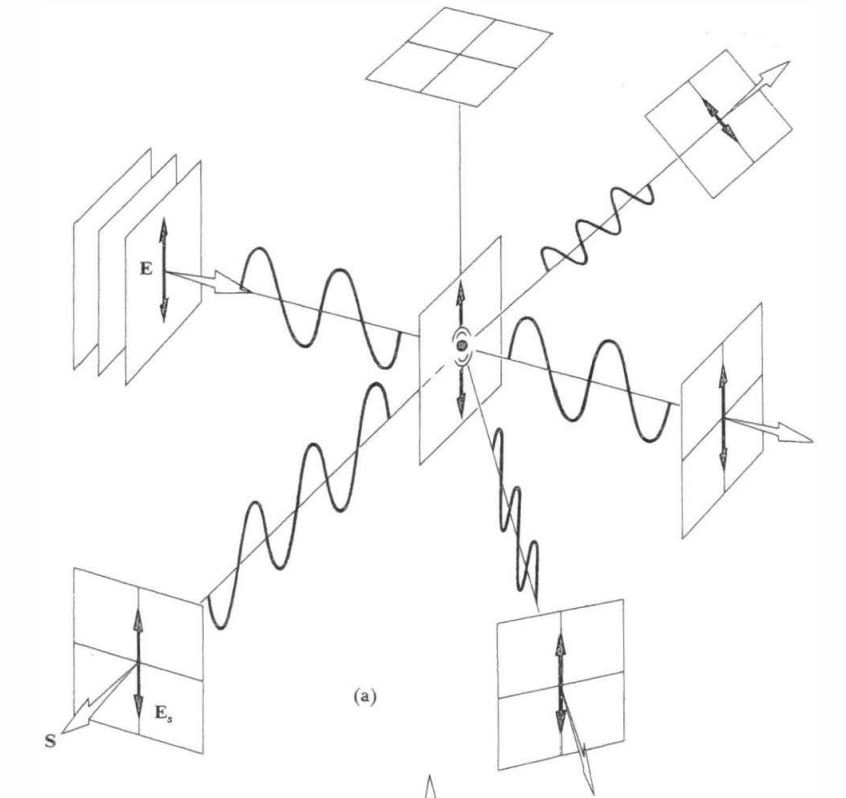
\includegraphics[width=0.4\textwidth]{prework.png}
    \caption{Scattering of polarised light by a molecule}
\end{figure}

Scattered light will only propagate in forward directions and not in the 
direction of the electric field. The magnitude will be equal in the 
directions orthogonal to the propagation of the electric field and decrease
as the angle between the propagation of the scattered wave and the propagation 
of the original wave's electric field is smaller.

\subsubsection{Question 2g}
Using
\begin{equation}
    I_1 = I_0 \cos^2{\theta}.
\end{equation}

a. 100\%
b. 50\%
c. 0\%
\subsection{Lab Book}
\subsubsection{Proper Attempt}

\begin{figure}[H]
    \centering
    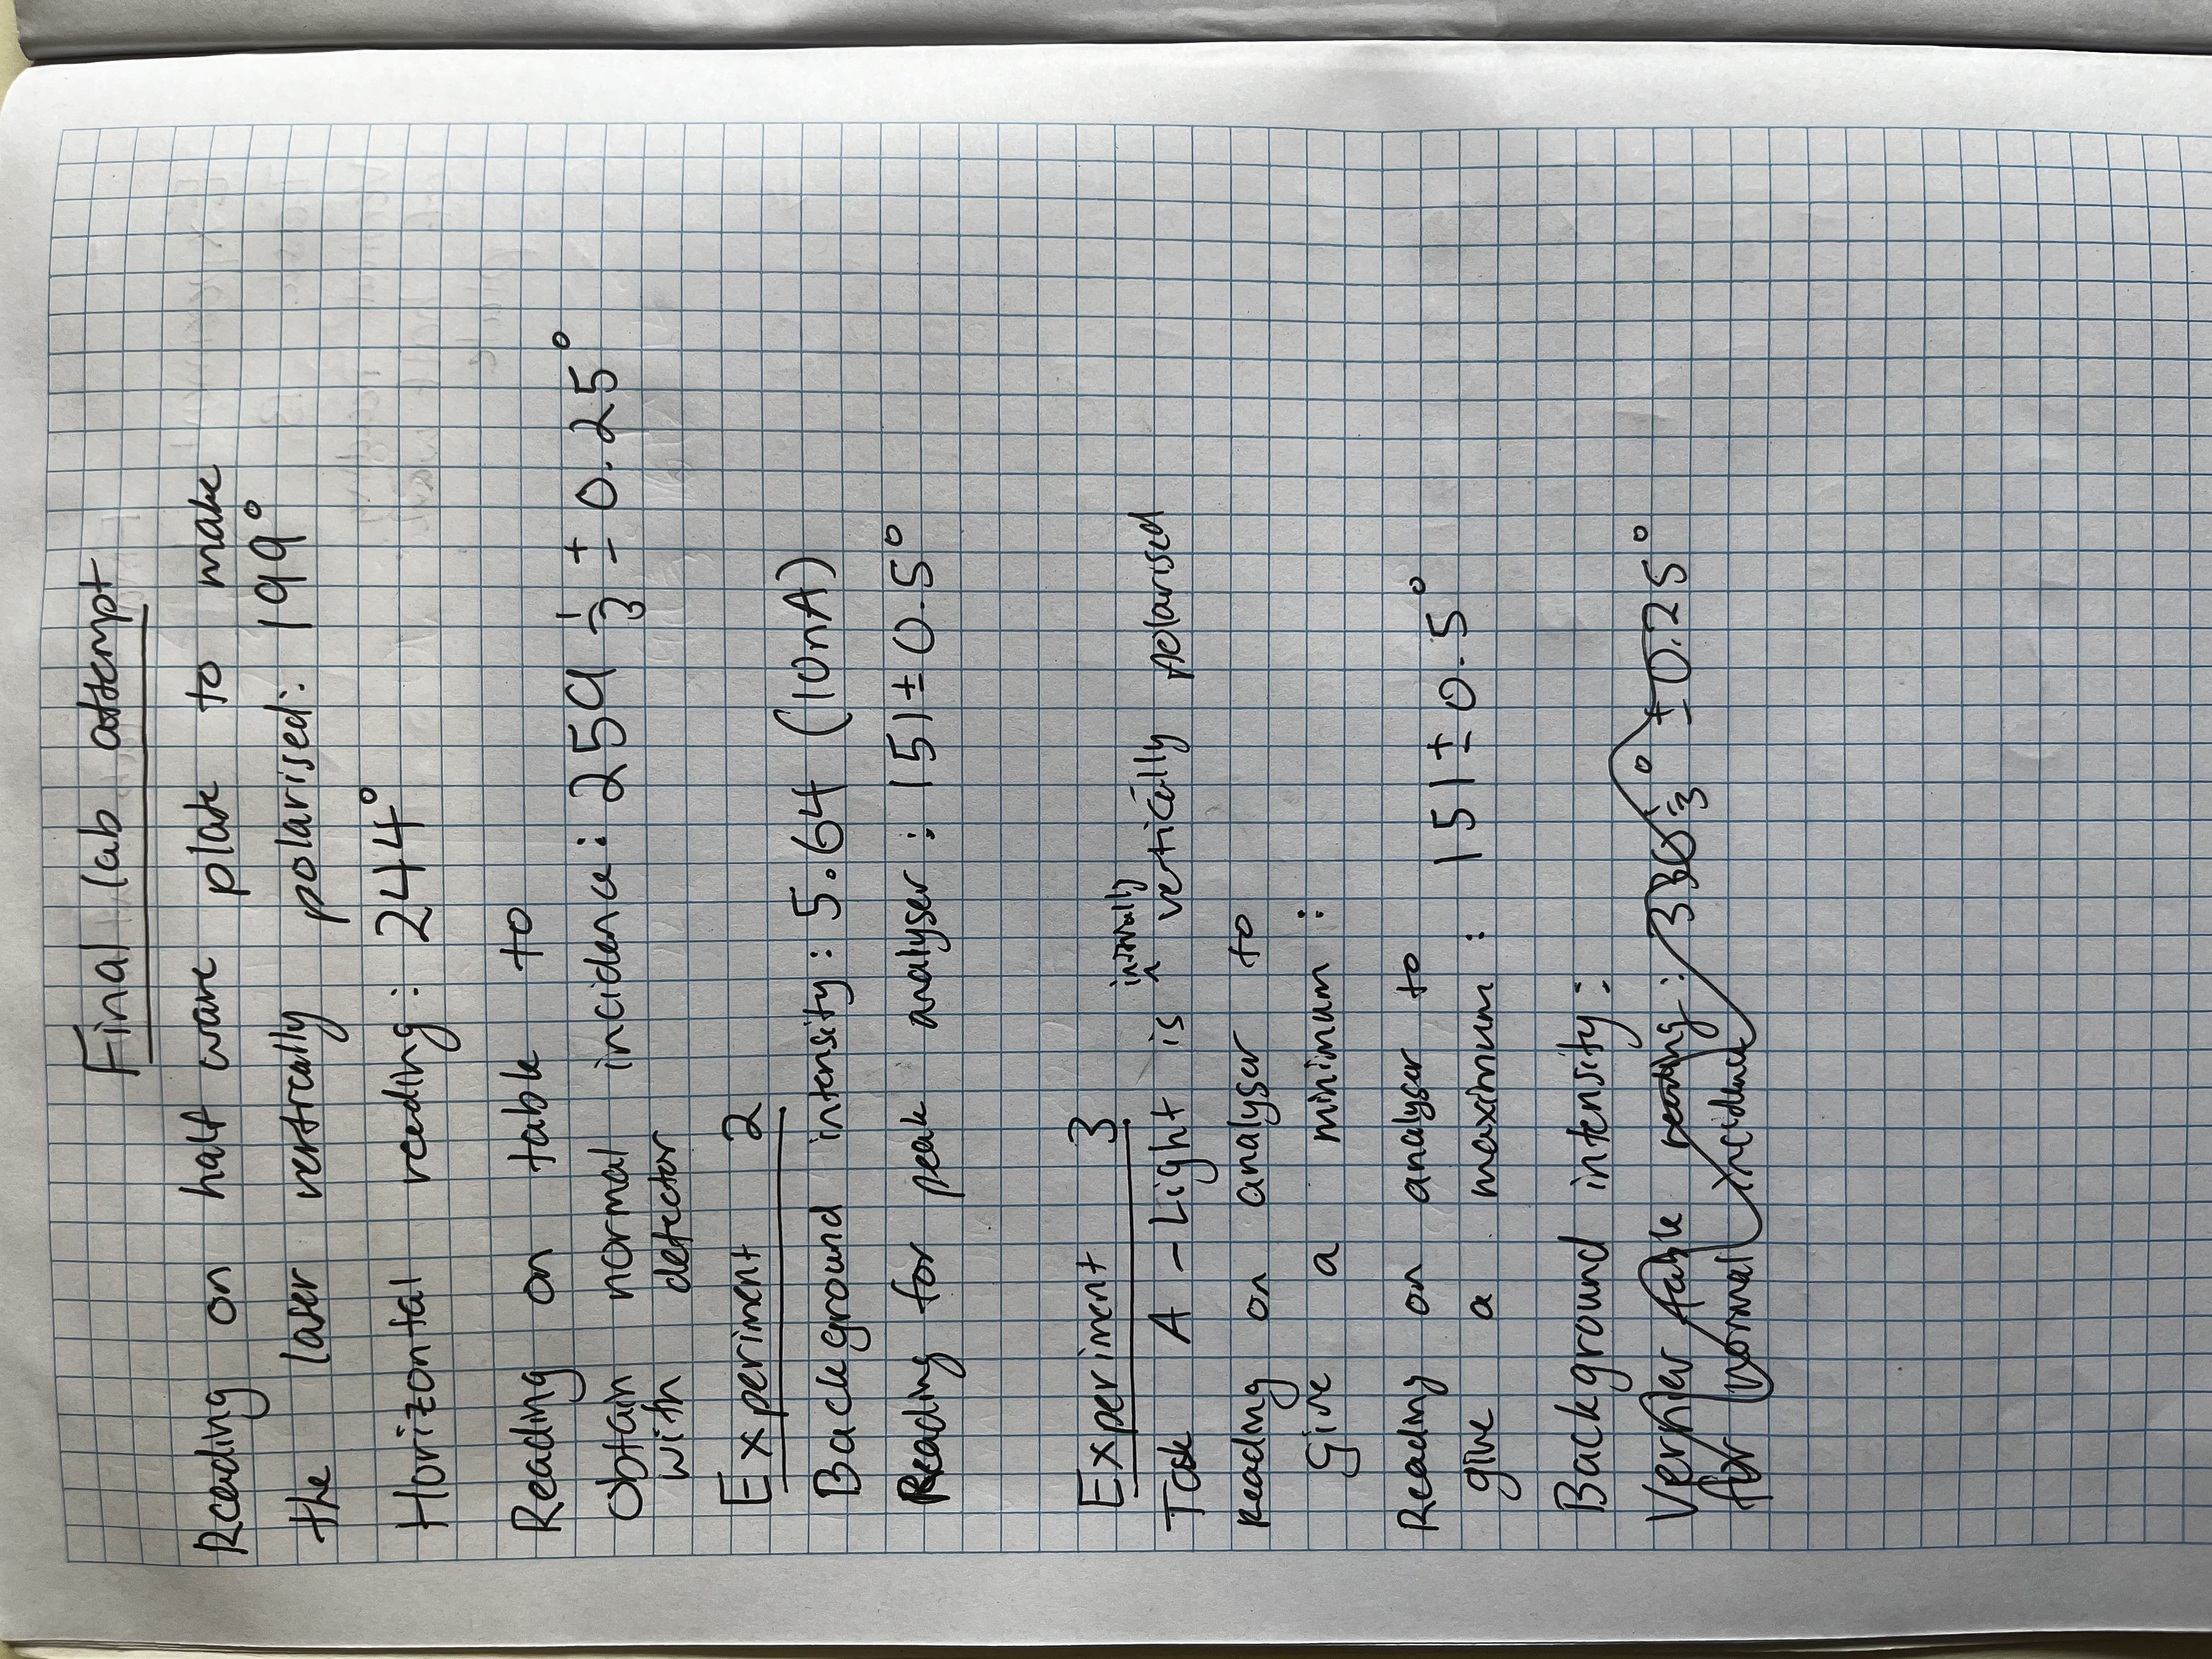
\includegraphics[width=0.5\textwidth,angle=270,origin=c]{labbook10.jpg}
    \hspace{0.5cm}
    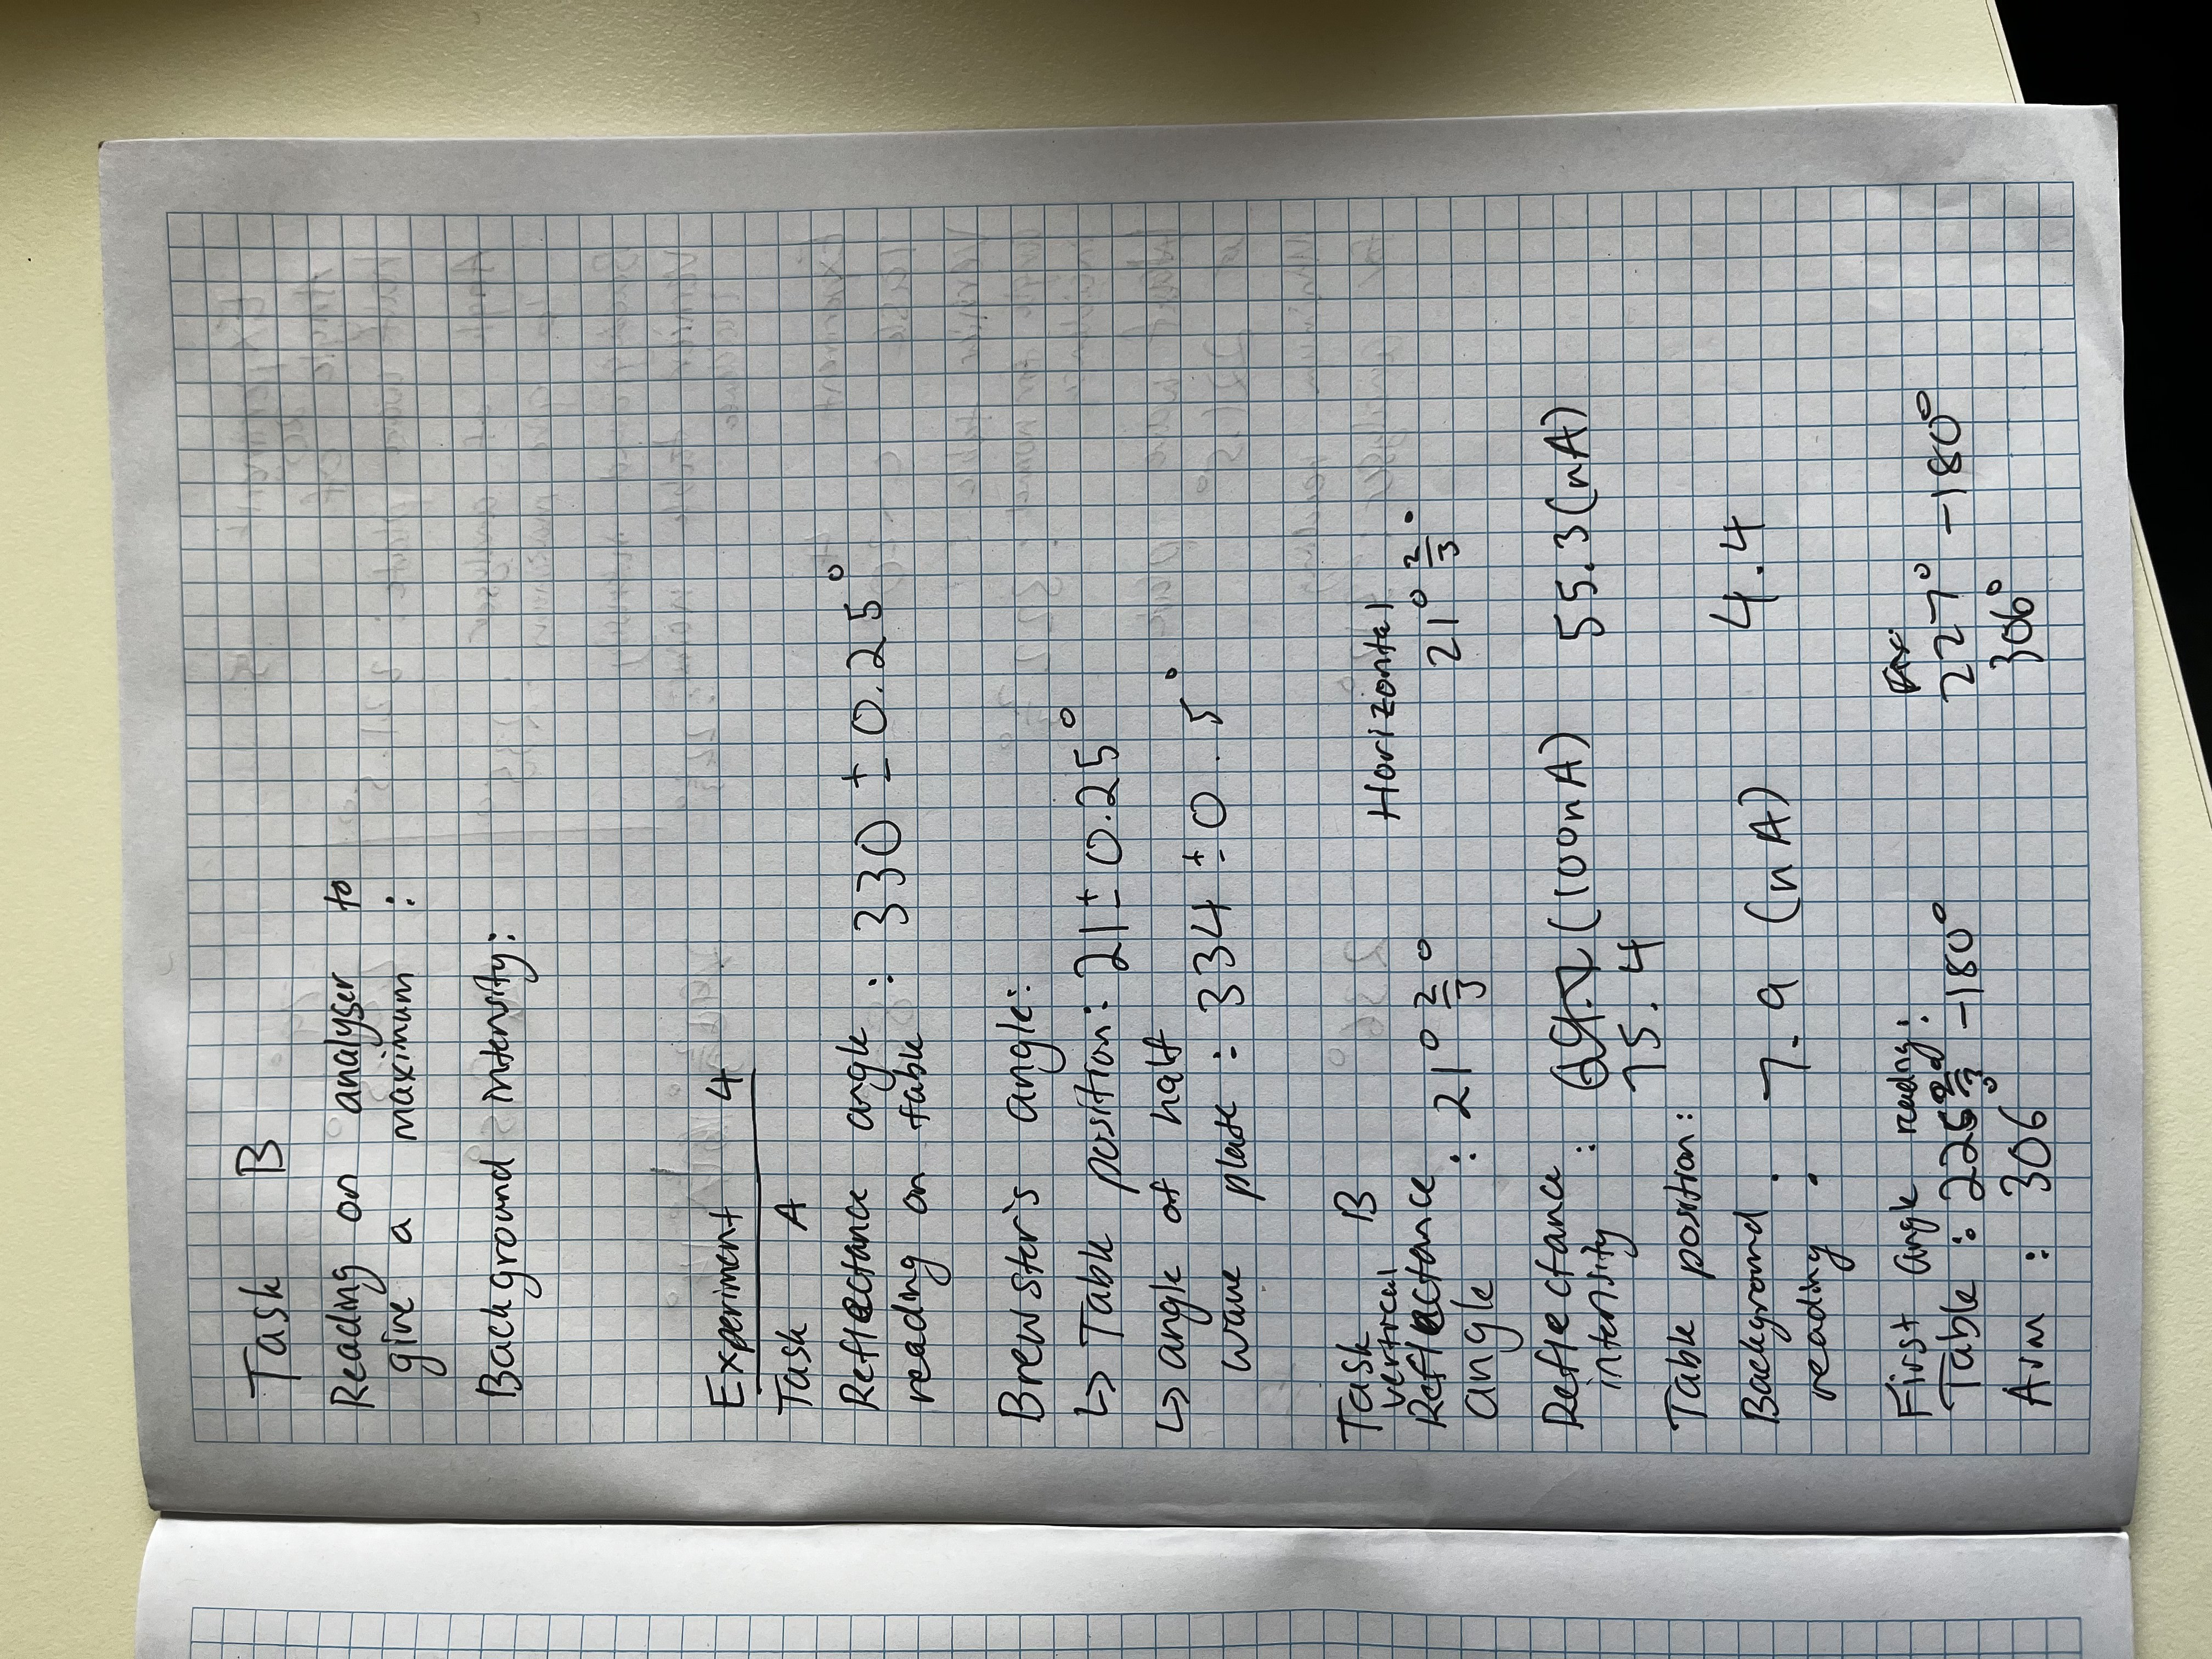
\includegraphics[width=0.5\textwidth,angle=270,origin=c]{labbook11.jpg}
    \vspace{0.5cm}
    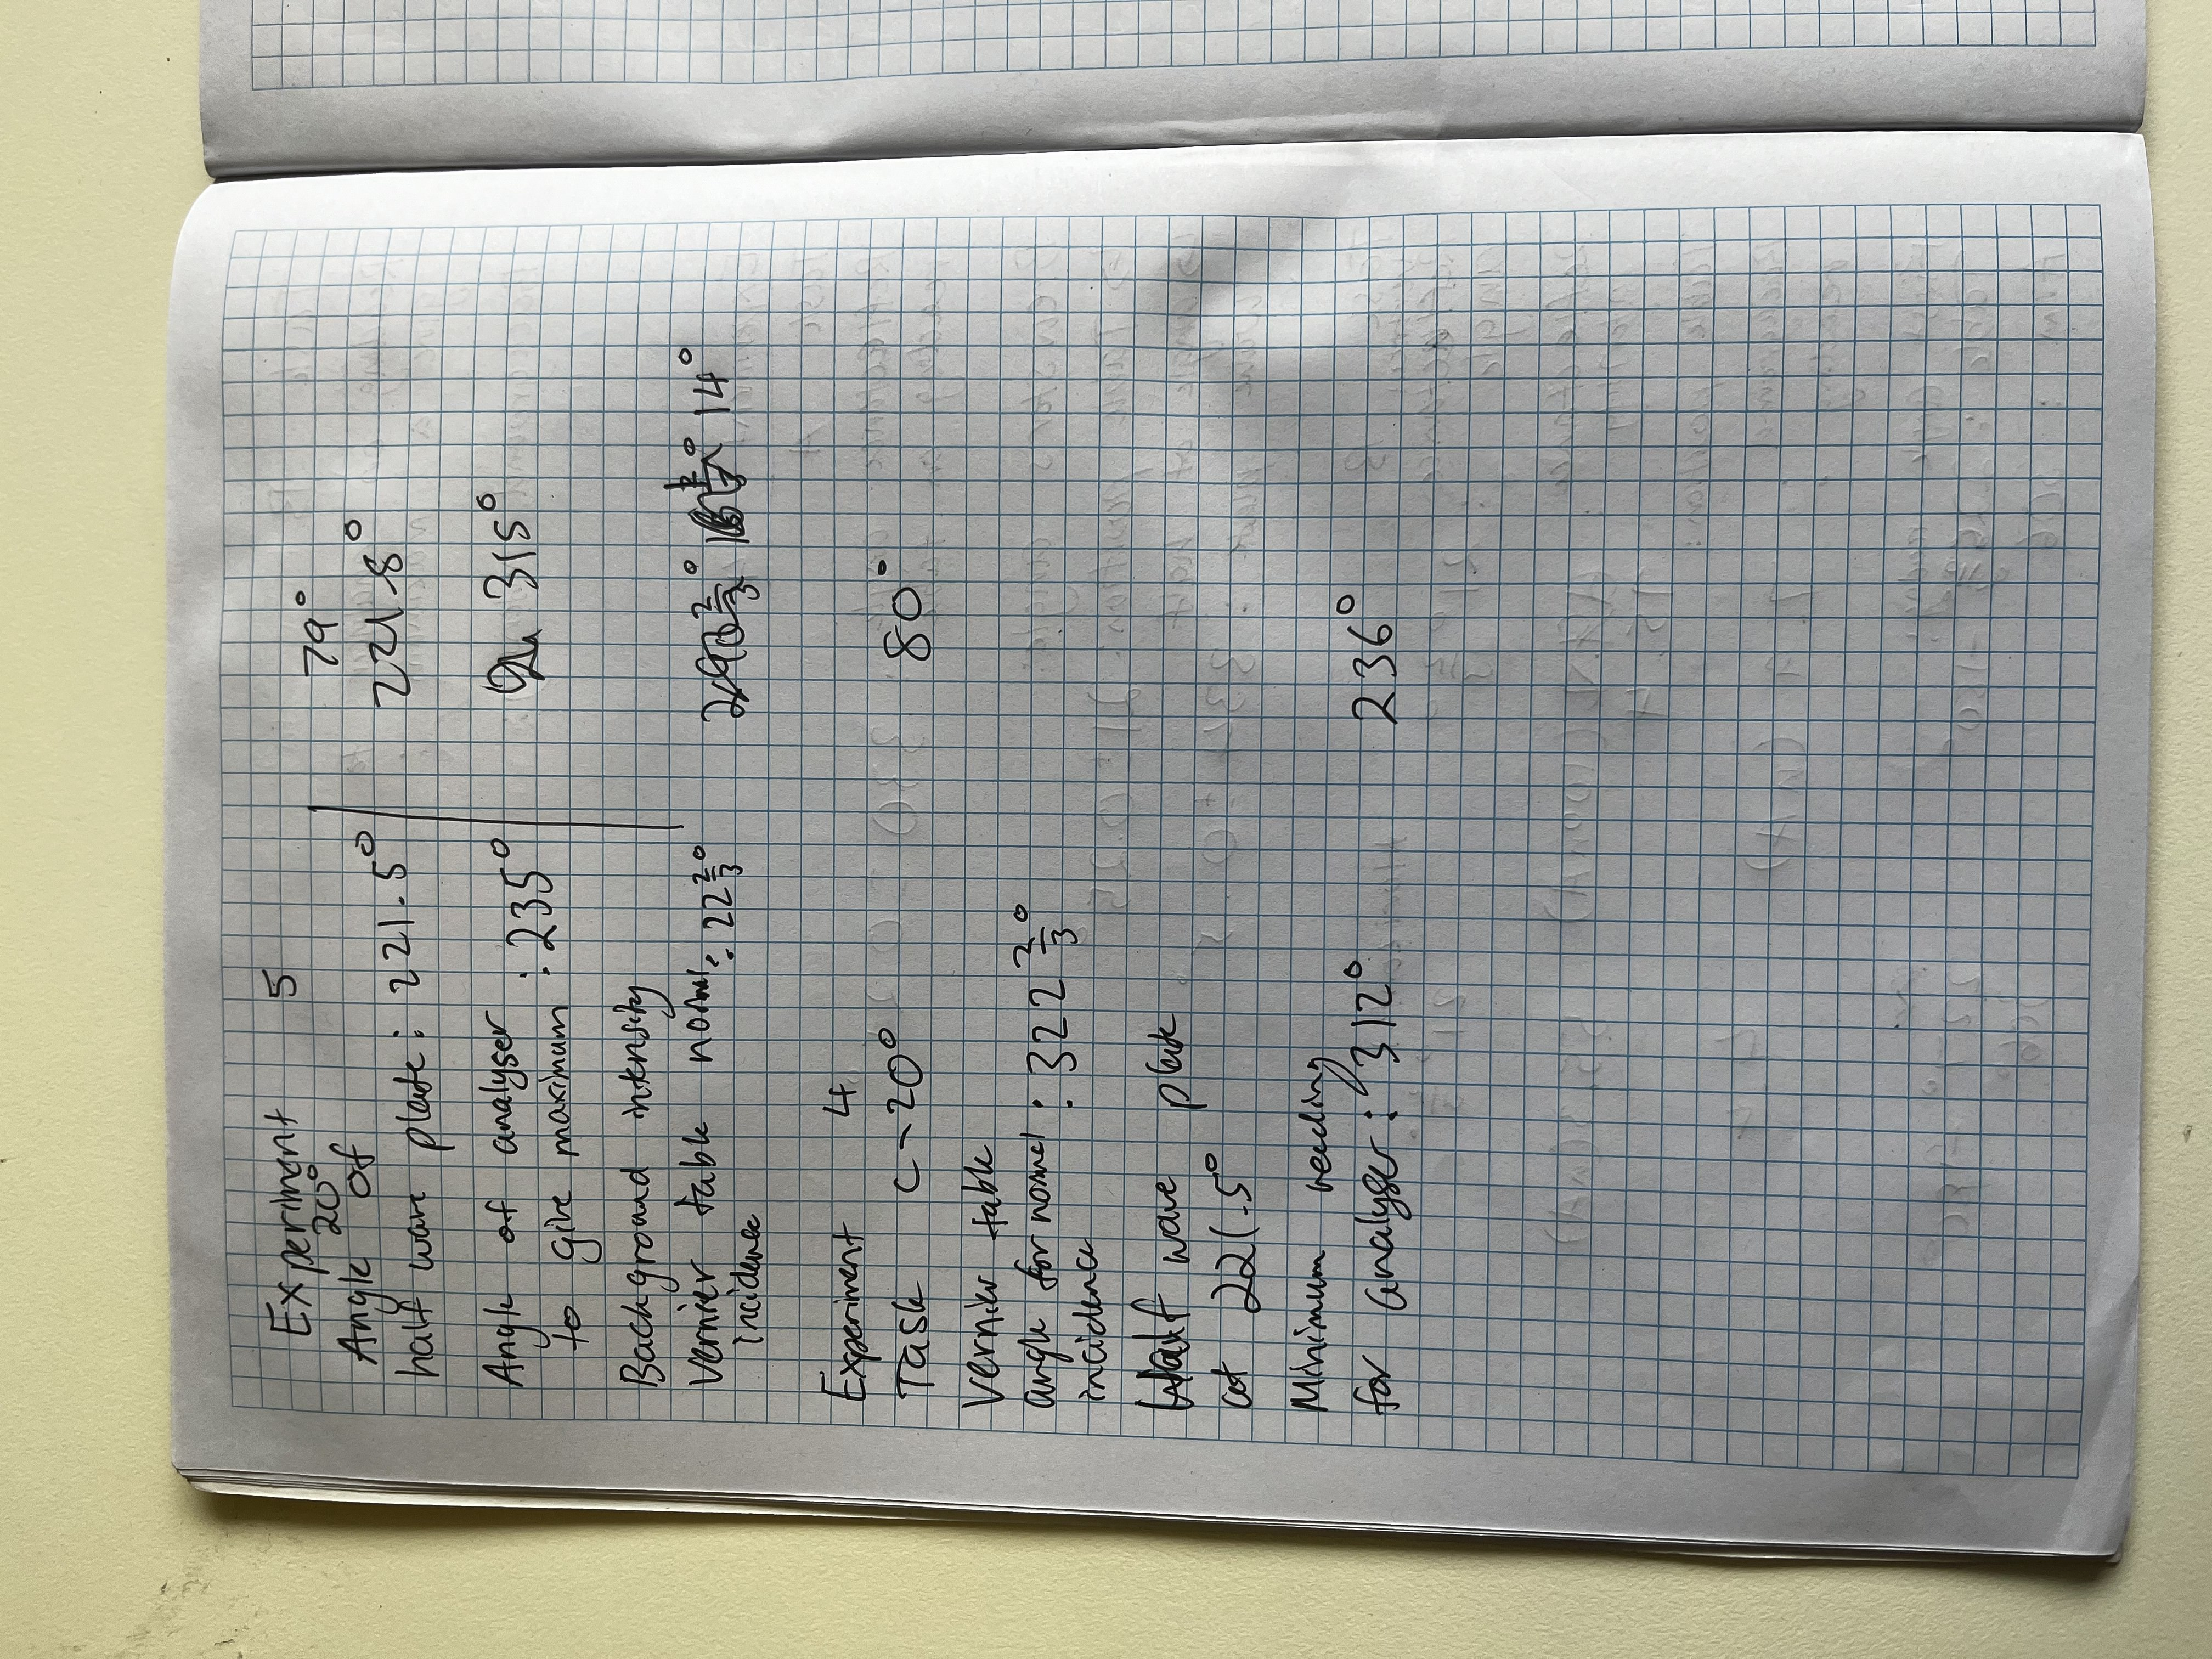
\includegraphics[width=0.5\textwidth,angle=270,origin=c]{labbook12.jpg}
\end{figure}


\subsubsection{Failed Attempts}
\begin{figure}[H]
    \centering
    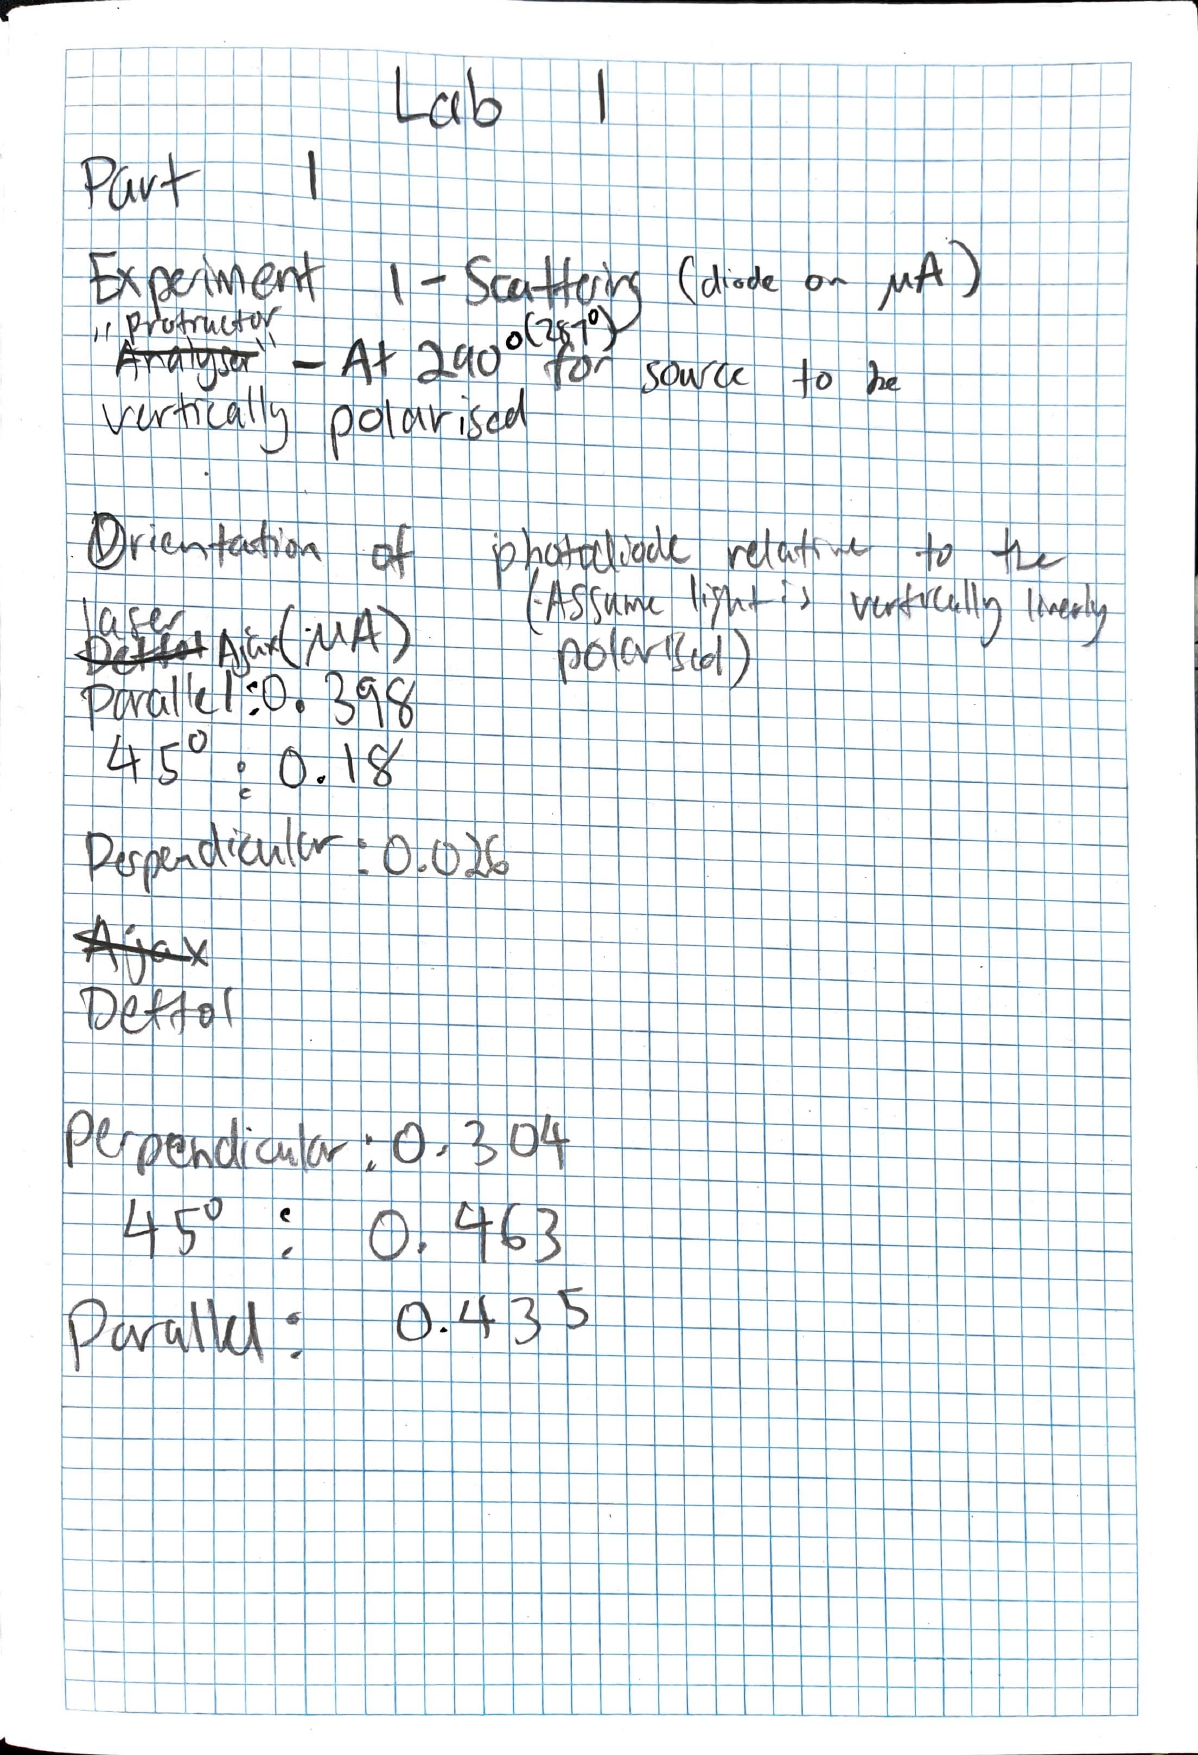
\includegraphics[width=0.2\textwidth]{labbook1.jpg}
    \hspace{0.5cm}
    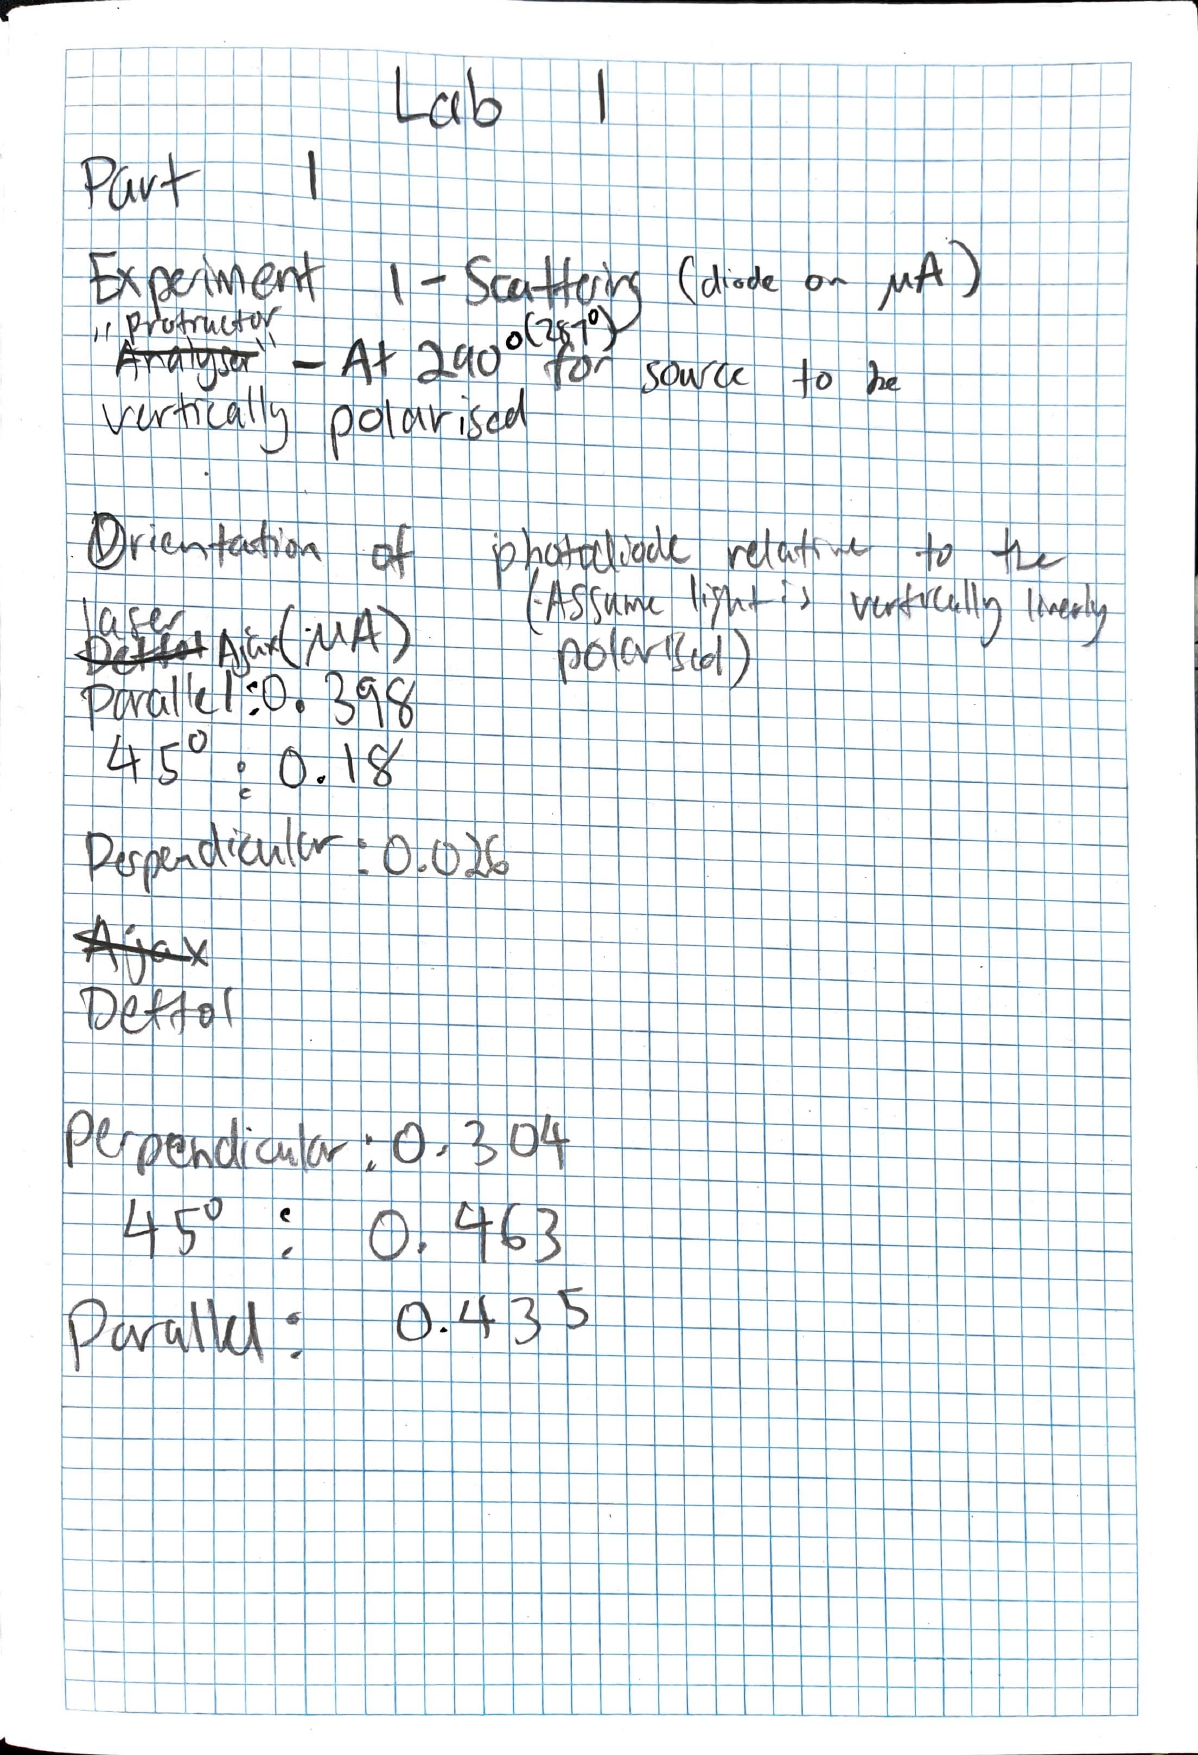
\includegraphics[width=0.2\textwidth]{labbook1.jpg}
    \vspace{0.5cm}
    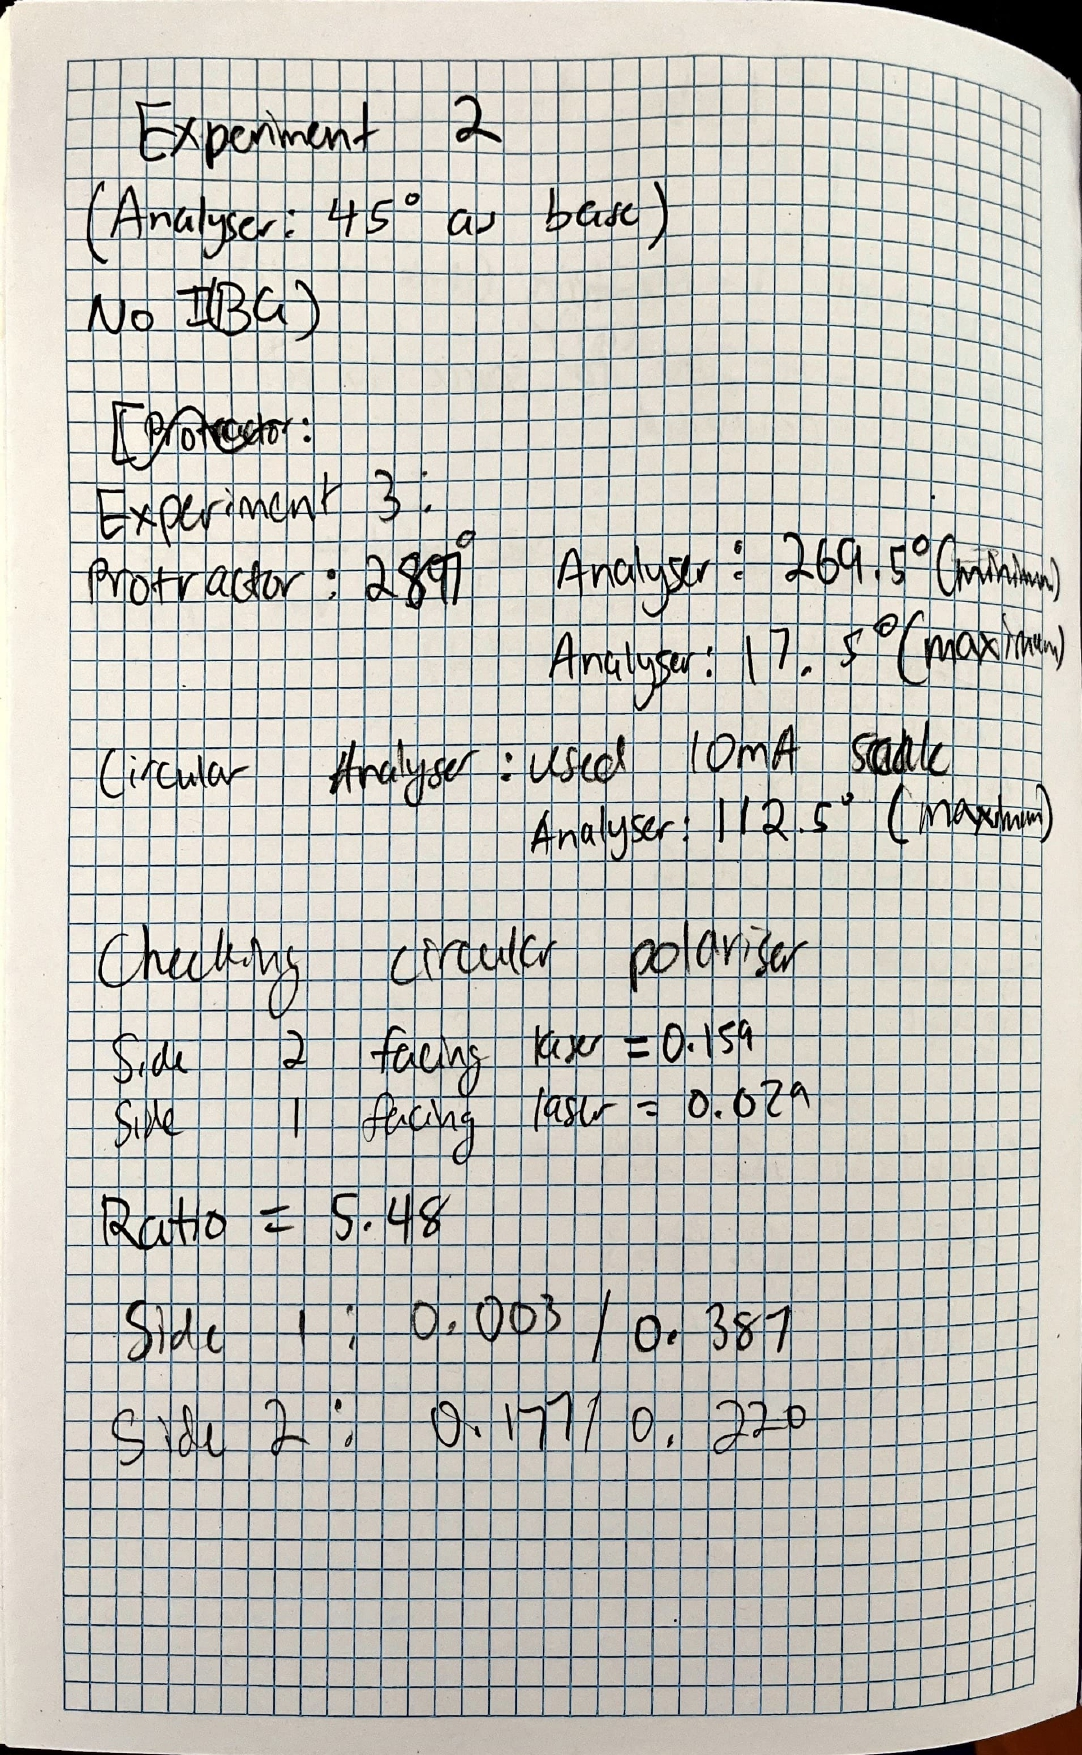
\includegraphics[width=0.2\textwidth]{labbook2.jpg}
    \hspace{0.5cm}
    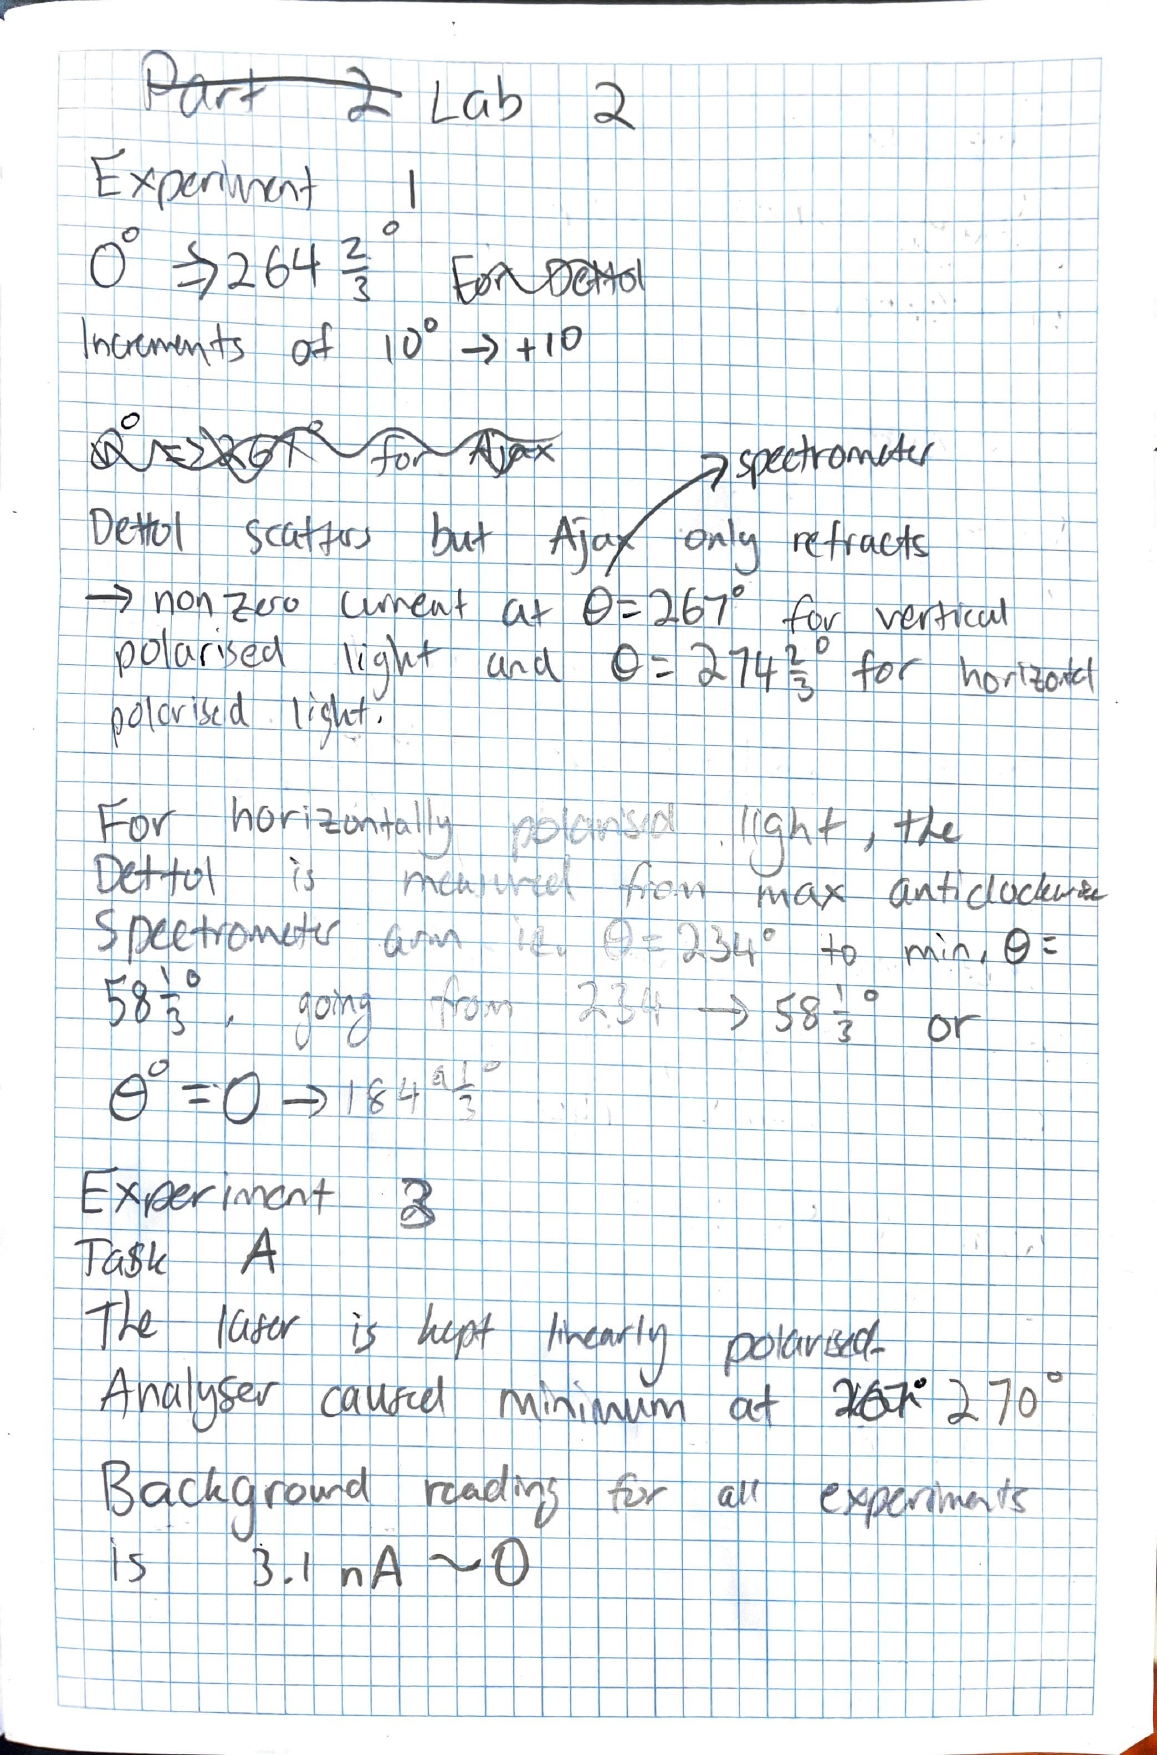
\includegraphics[width=0.2\textwidth]{labbook4.jpg}
    \vspace{0.5cm}
    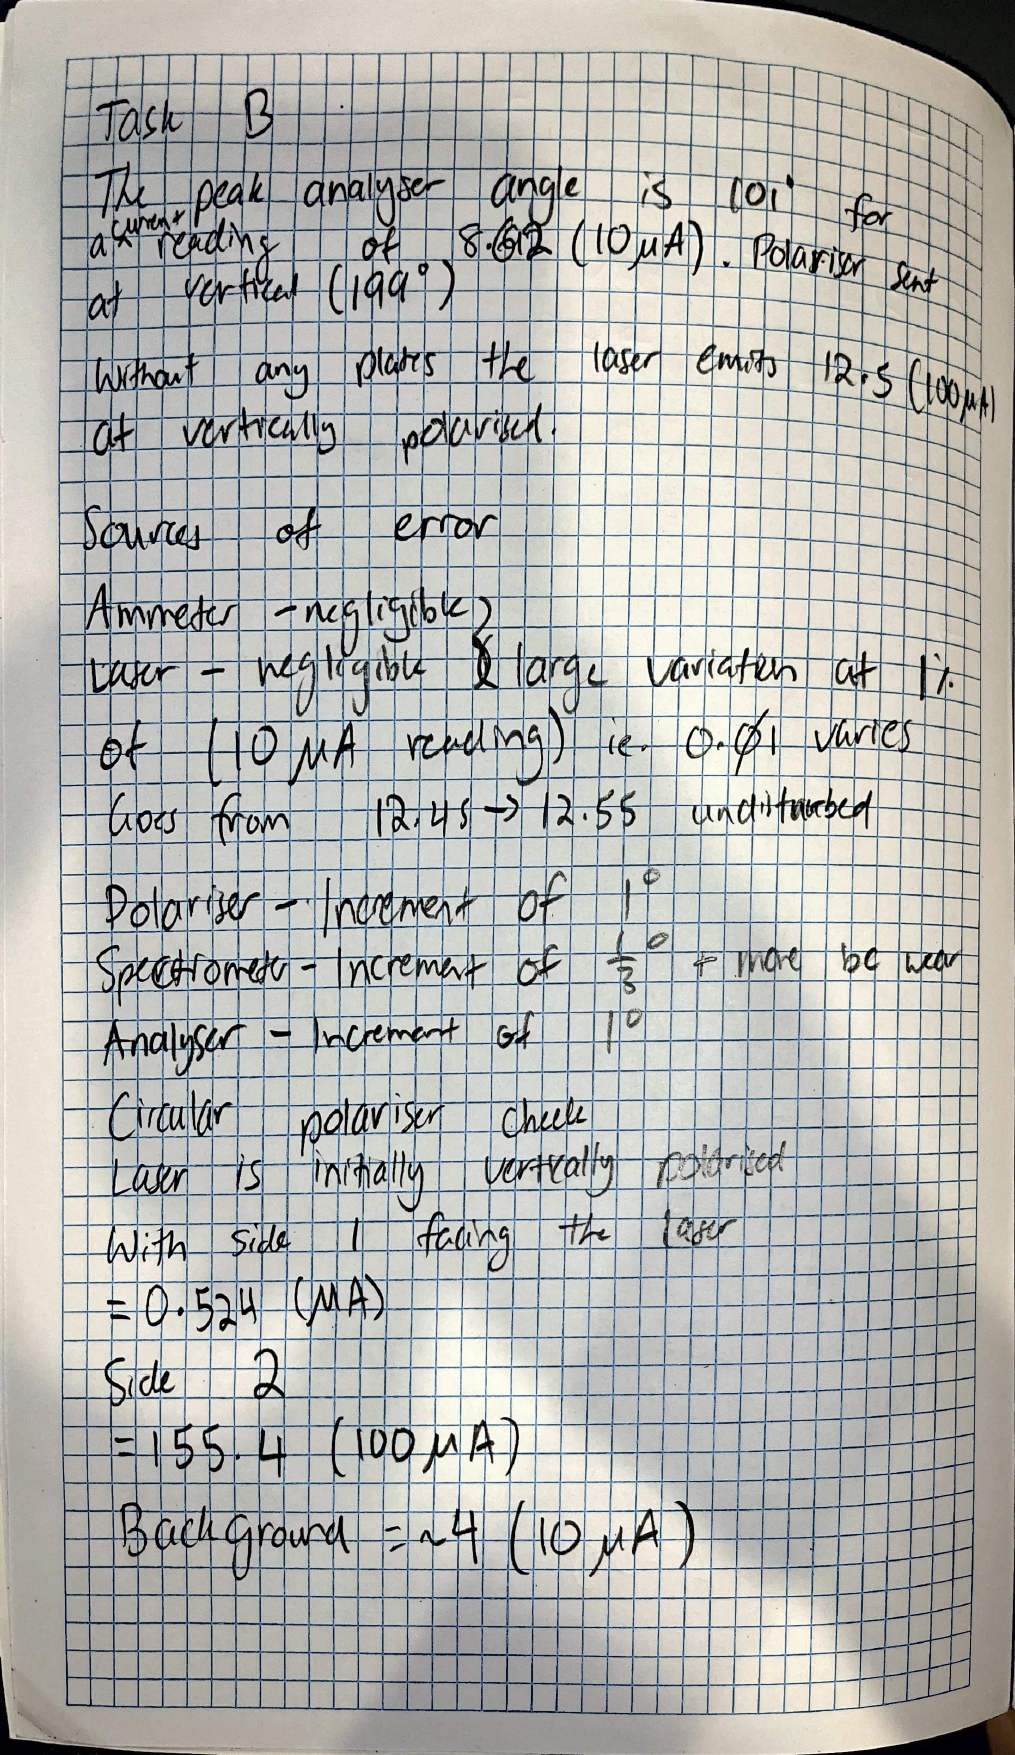
\includegraphics[width=0.2\textwidth]{labbook3.jpg}
    \hspace{0.5cm}
    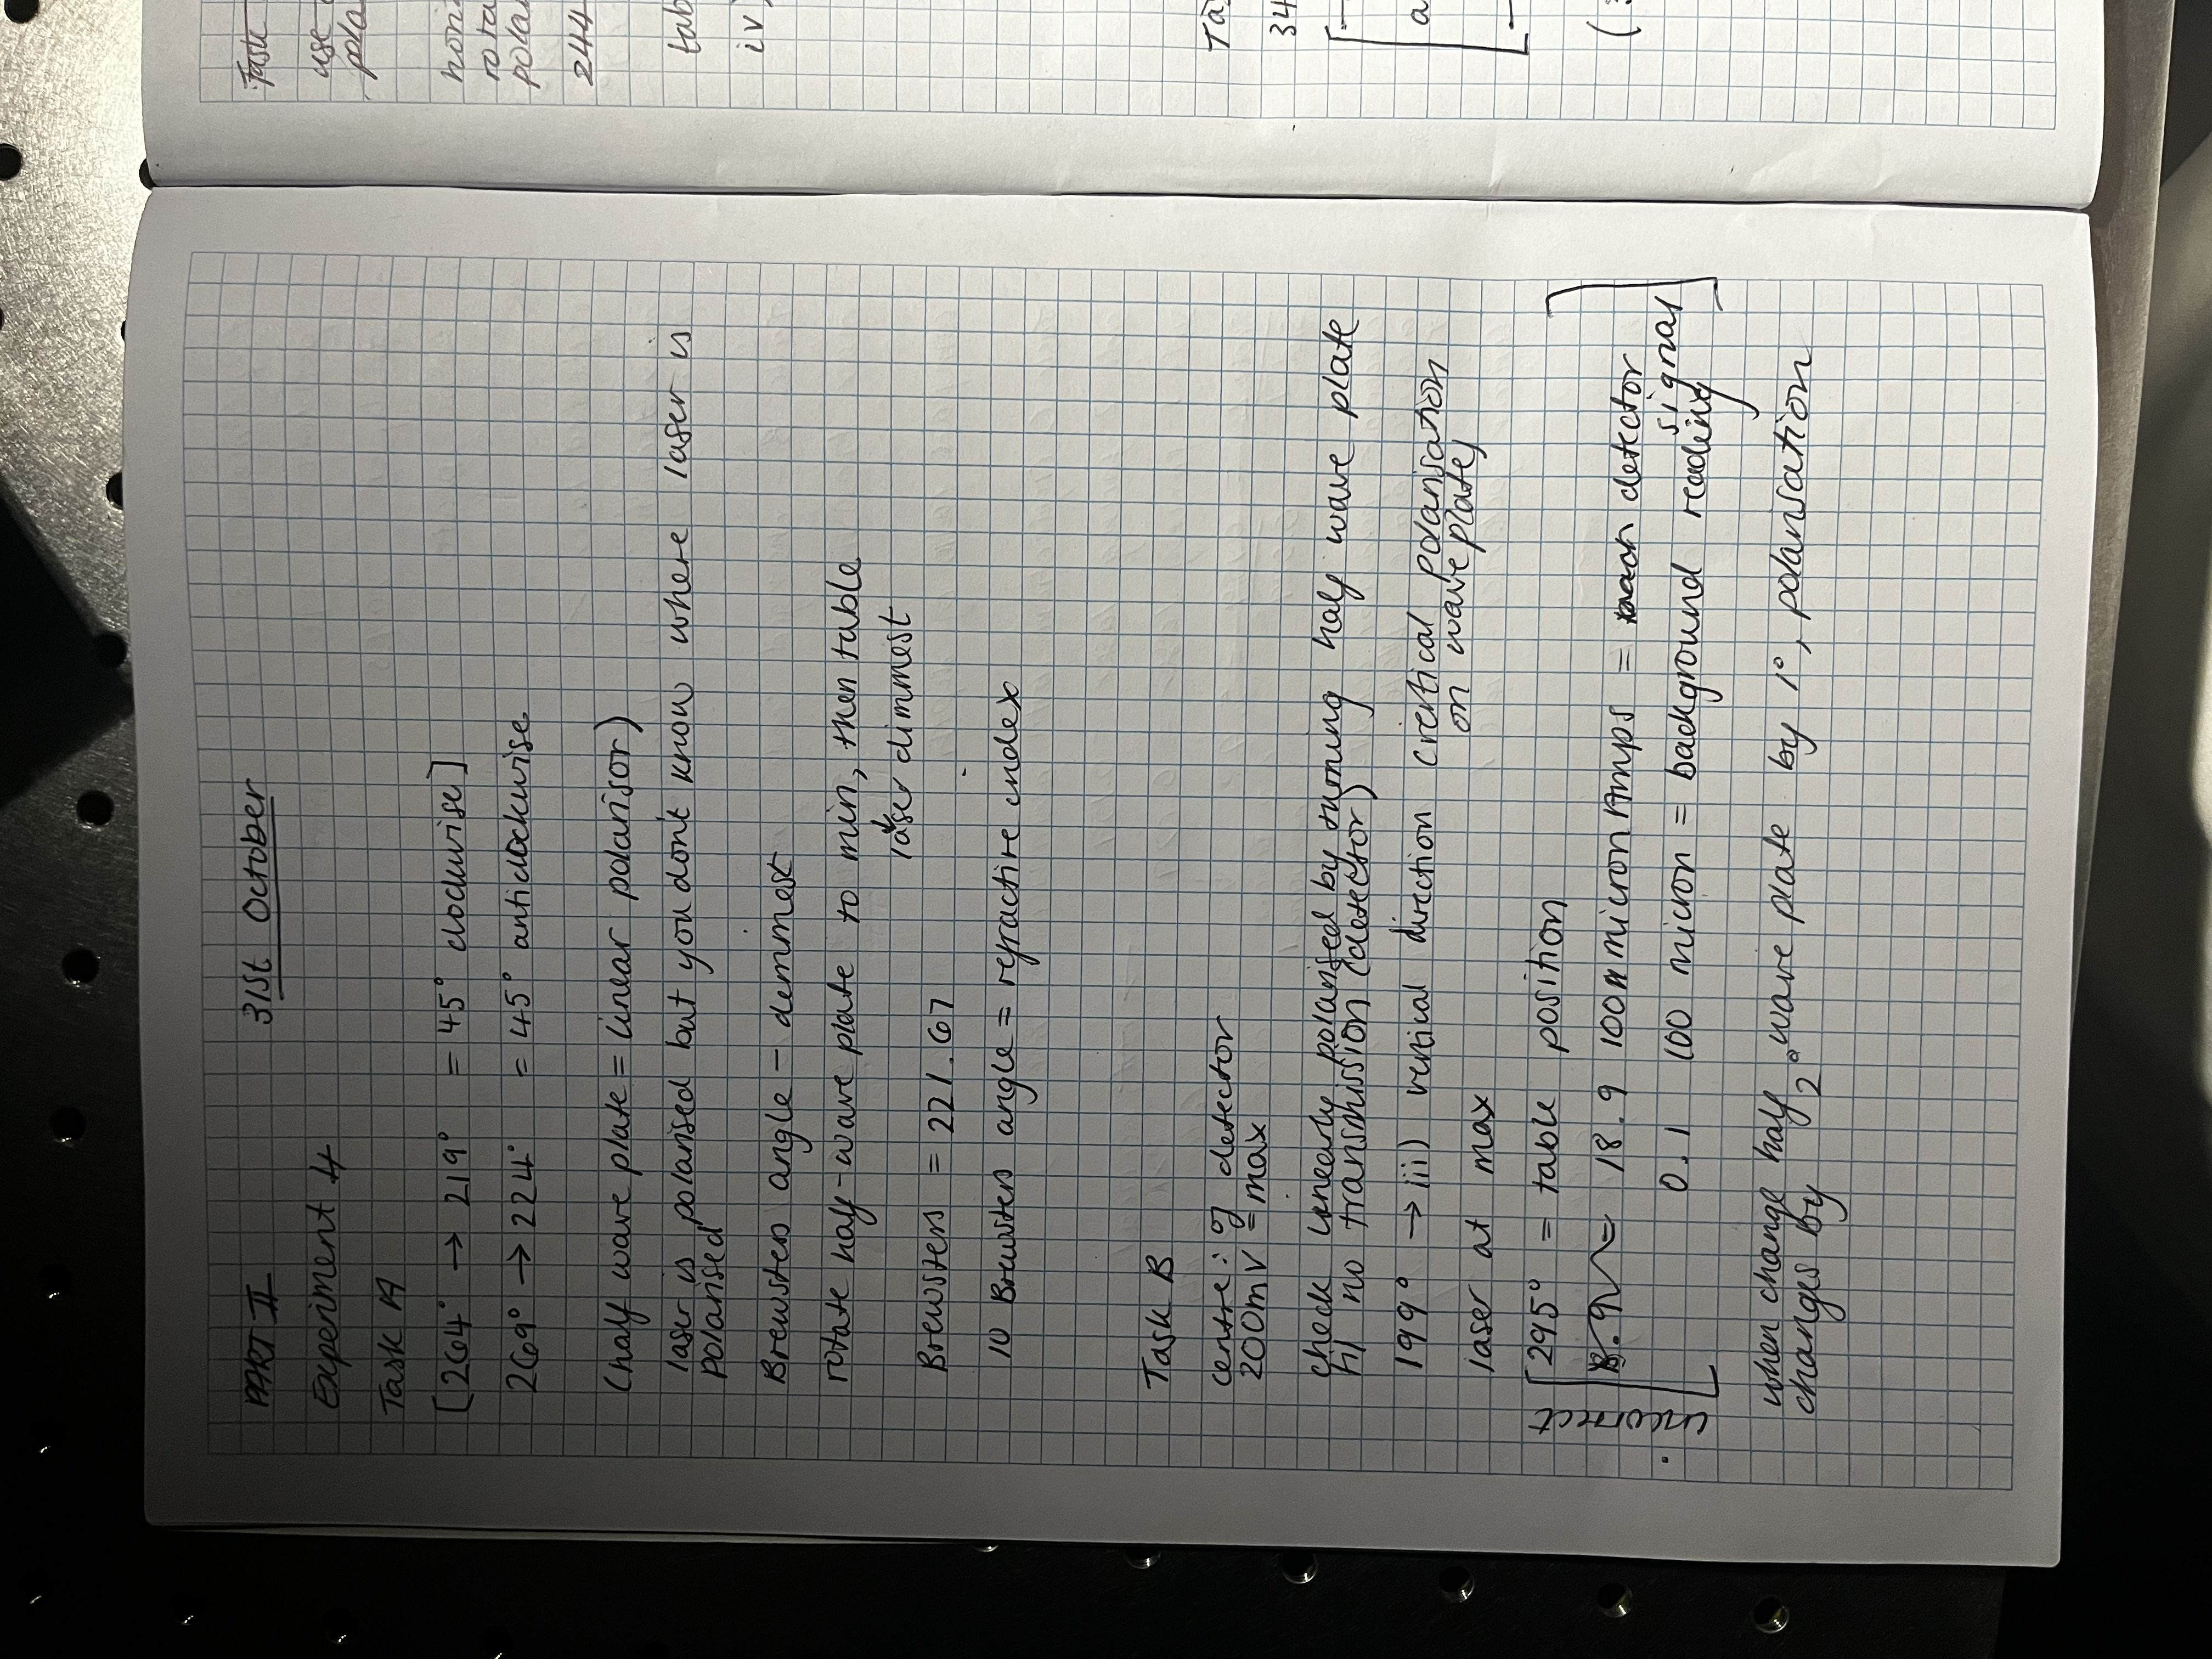
\includegraphics[width=0.2\textwidth,angle=270,origin=c]{labbook8.jpg}
    \vspace{0.5cm}
    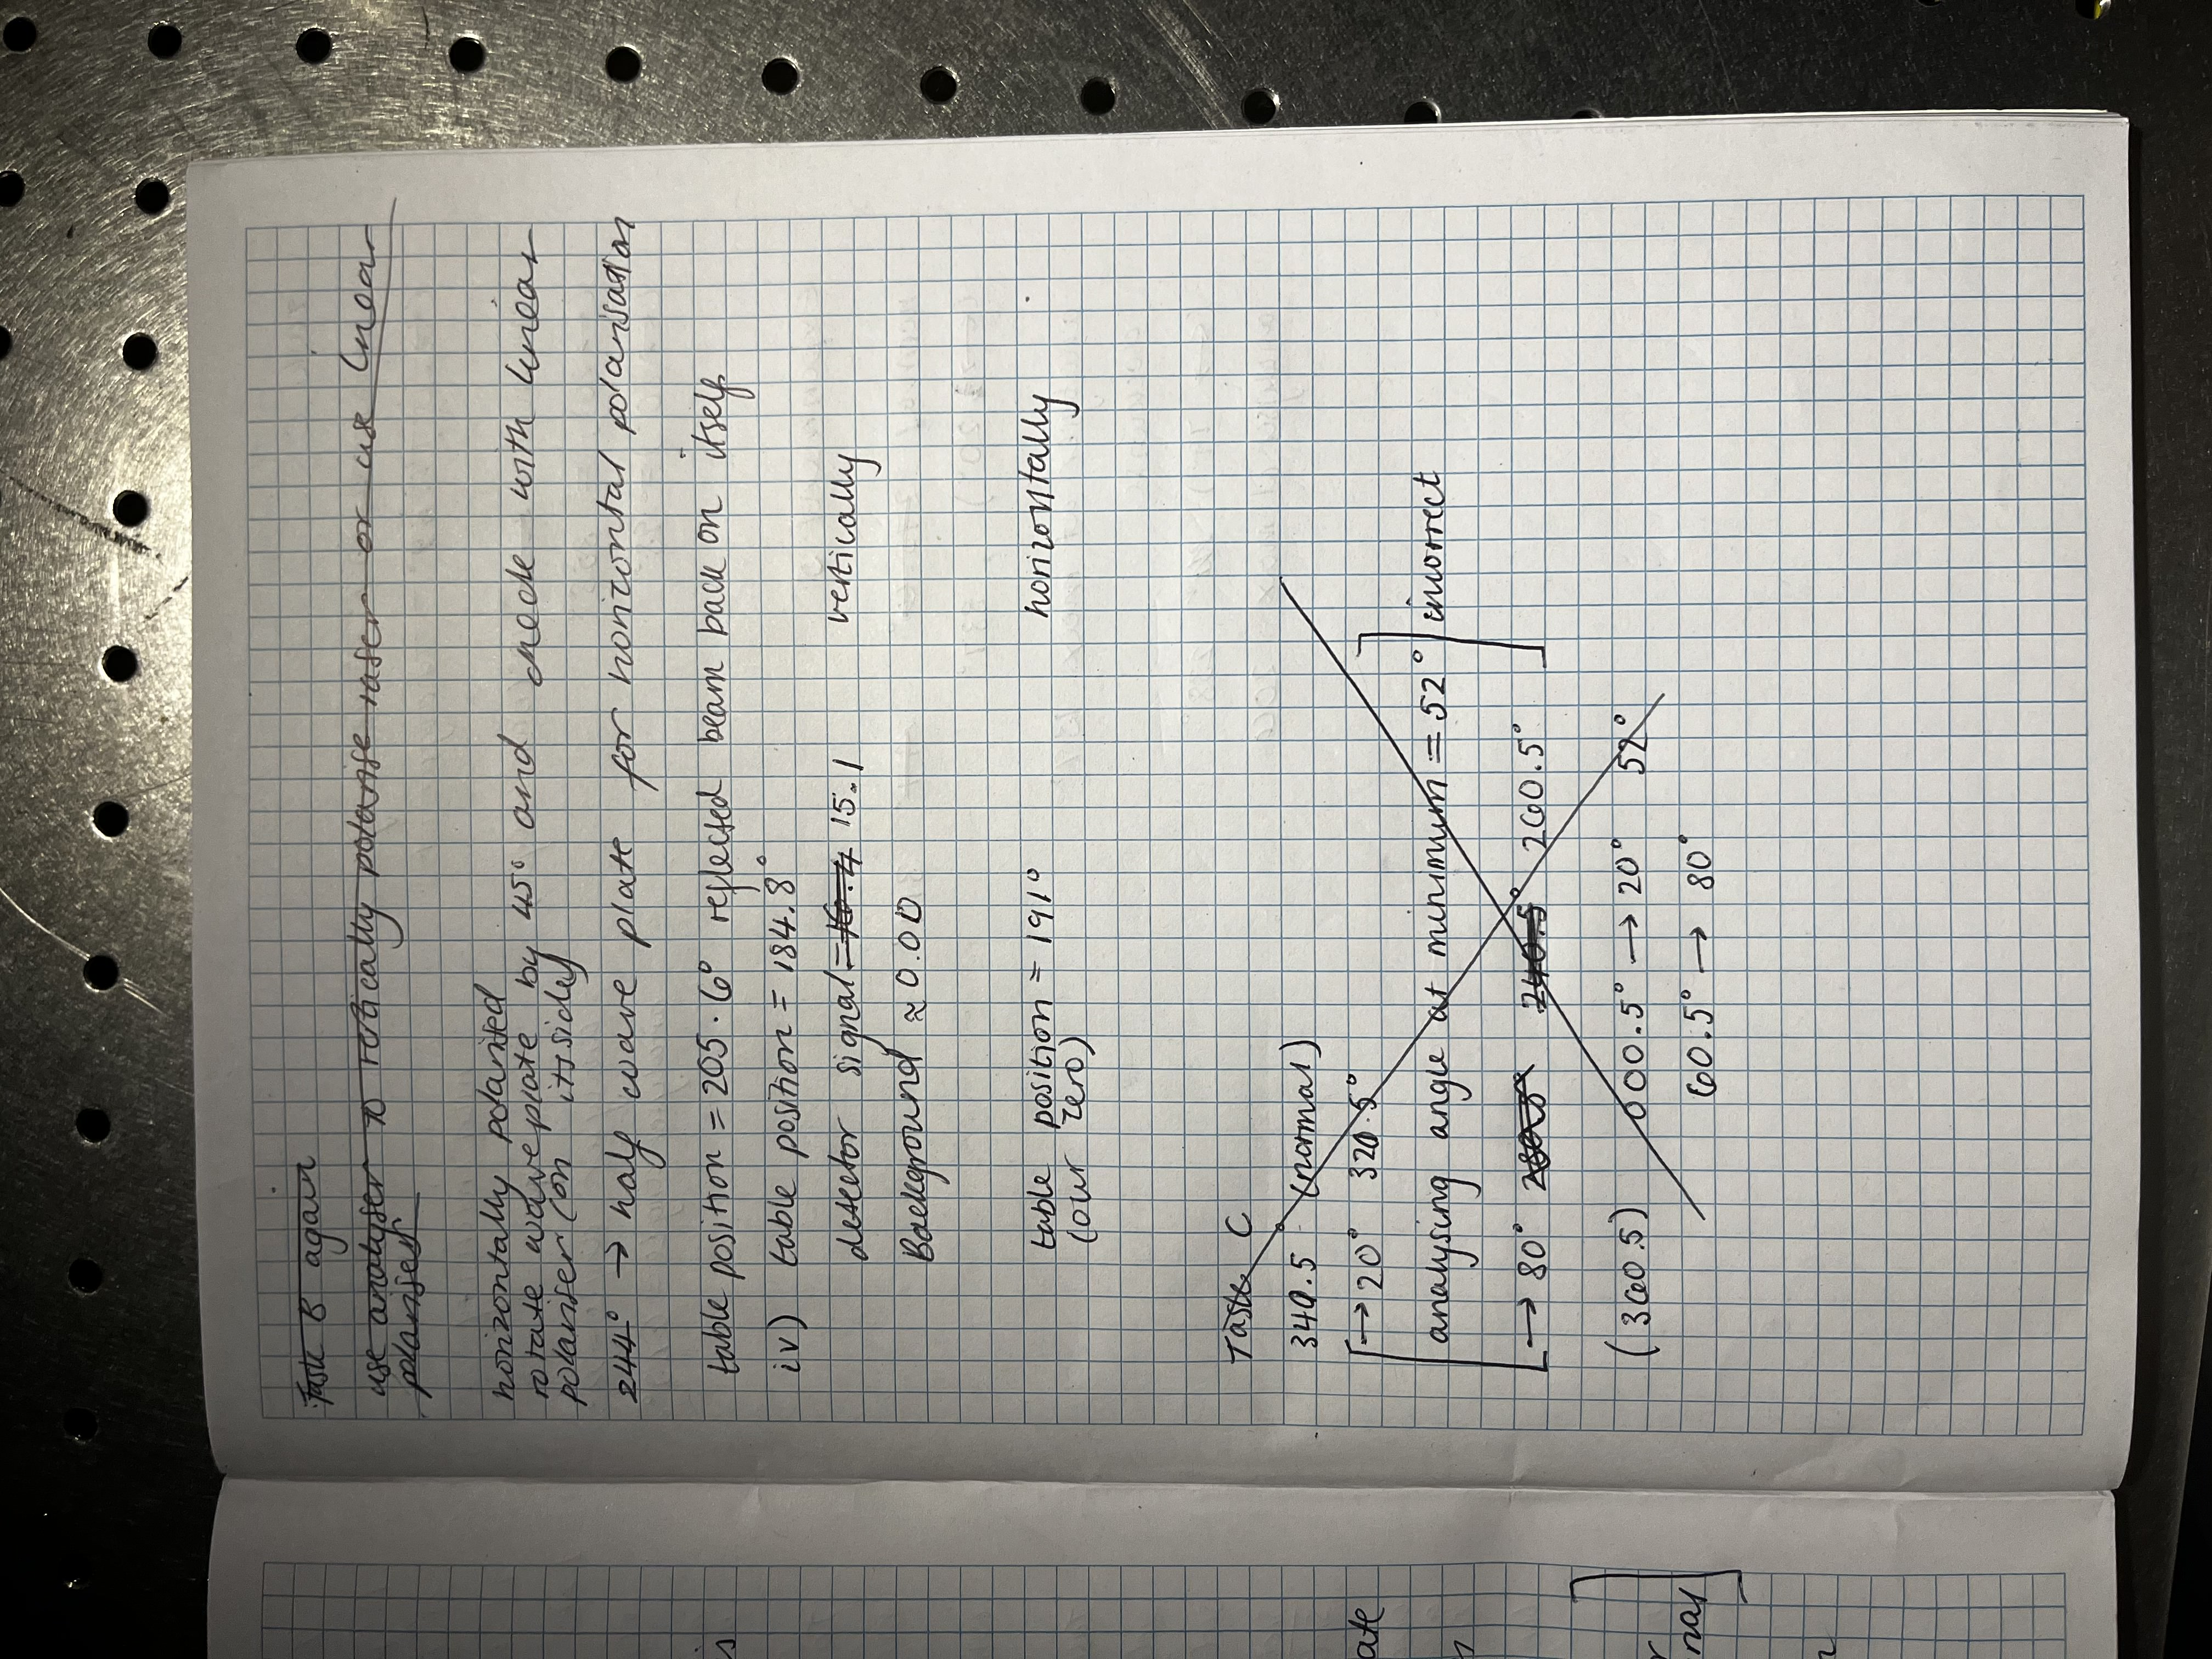
\includegraphics[width=0.2\textwidth,angle=270,origin=c]{labbook9.jpg}
\end{figure}

\subsection{Derivations}
\subsubsection{Quarter wave plate using Jones matrices}\label{eq:derivation}
\begin{figure}[H]
    \centering
    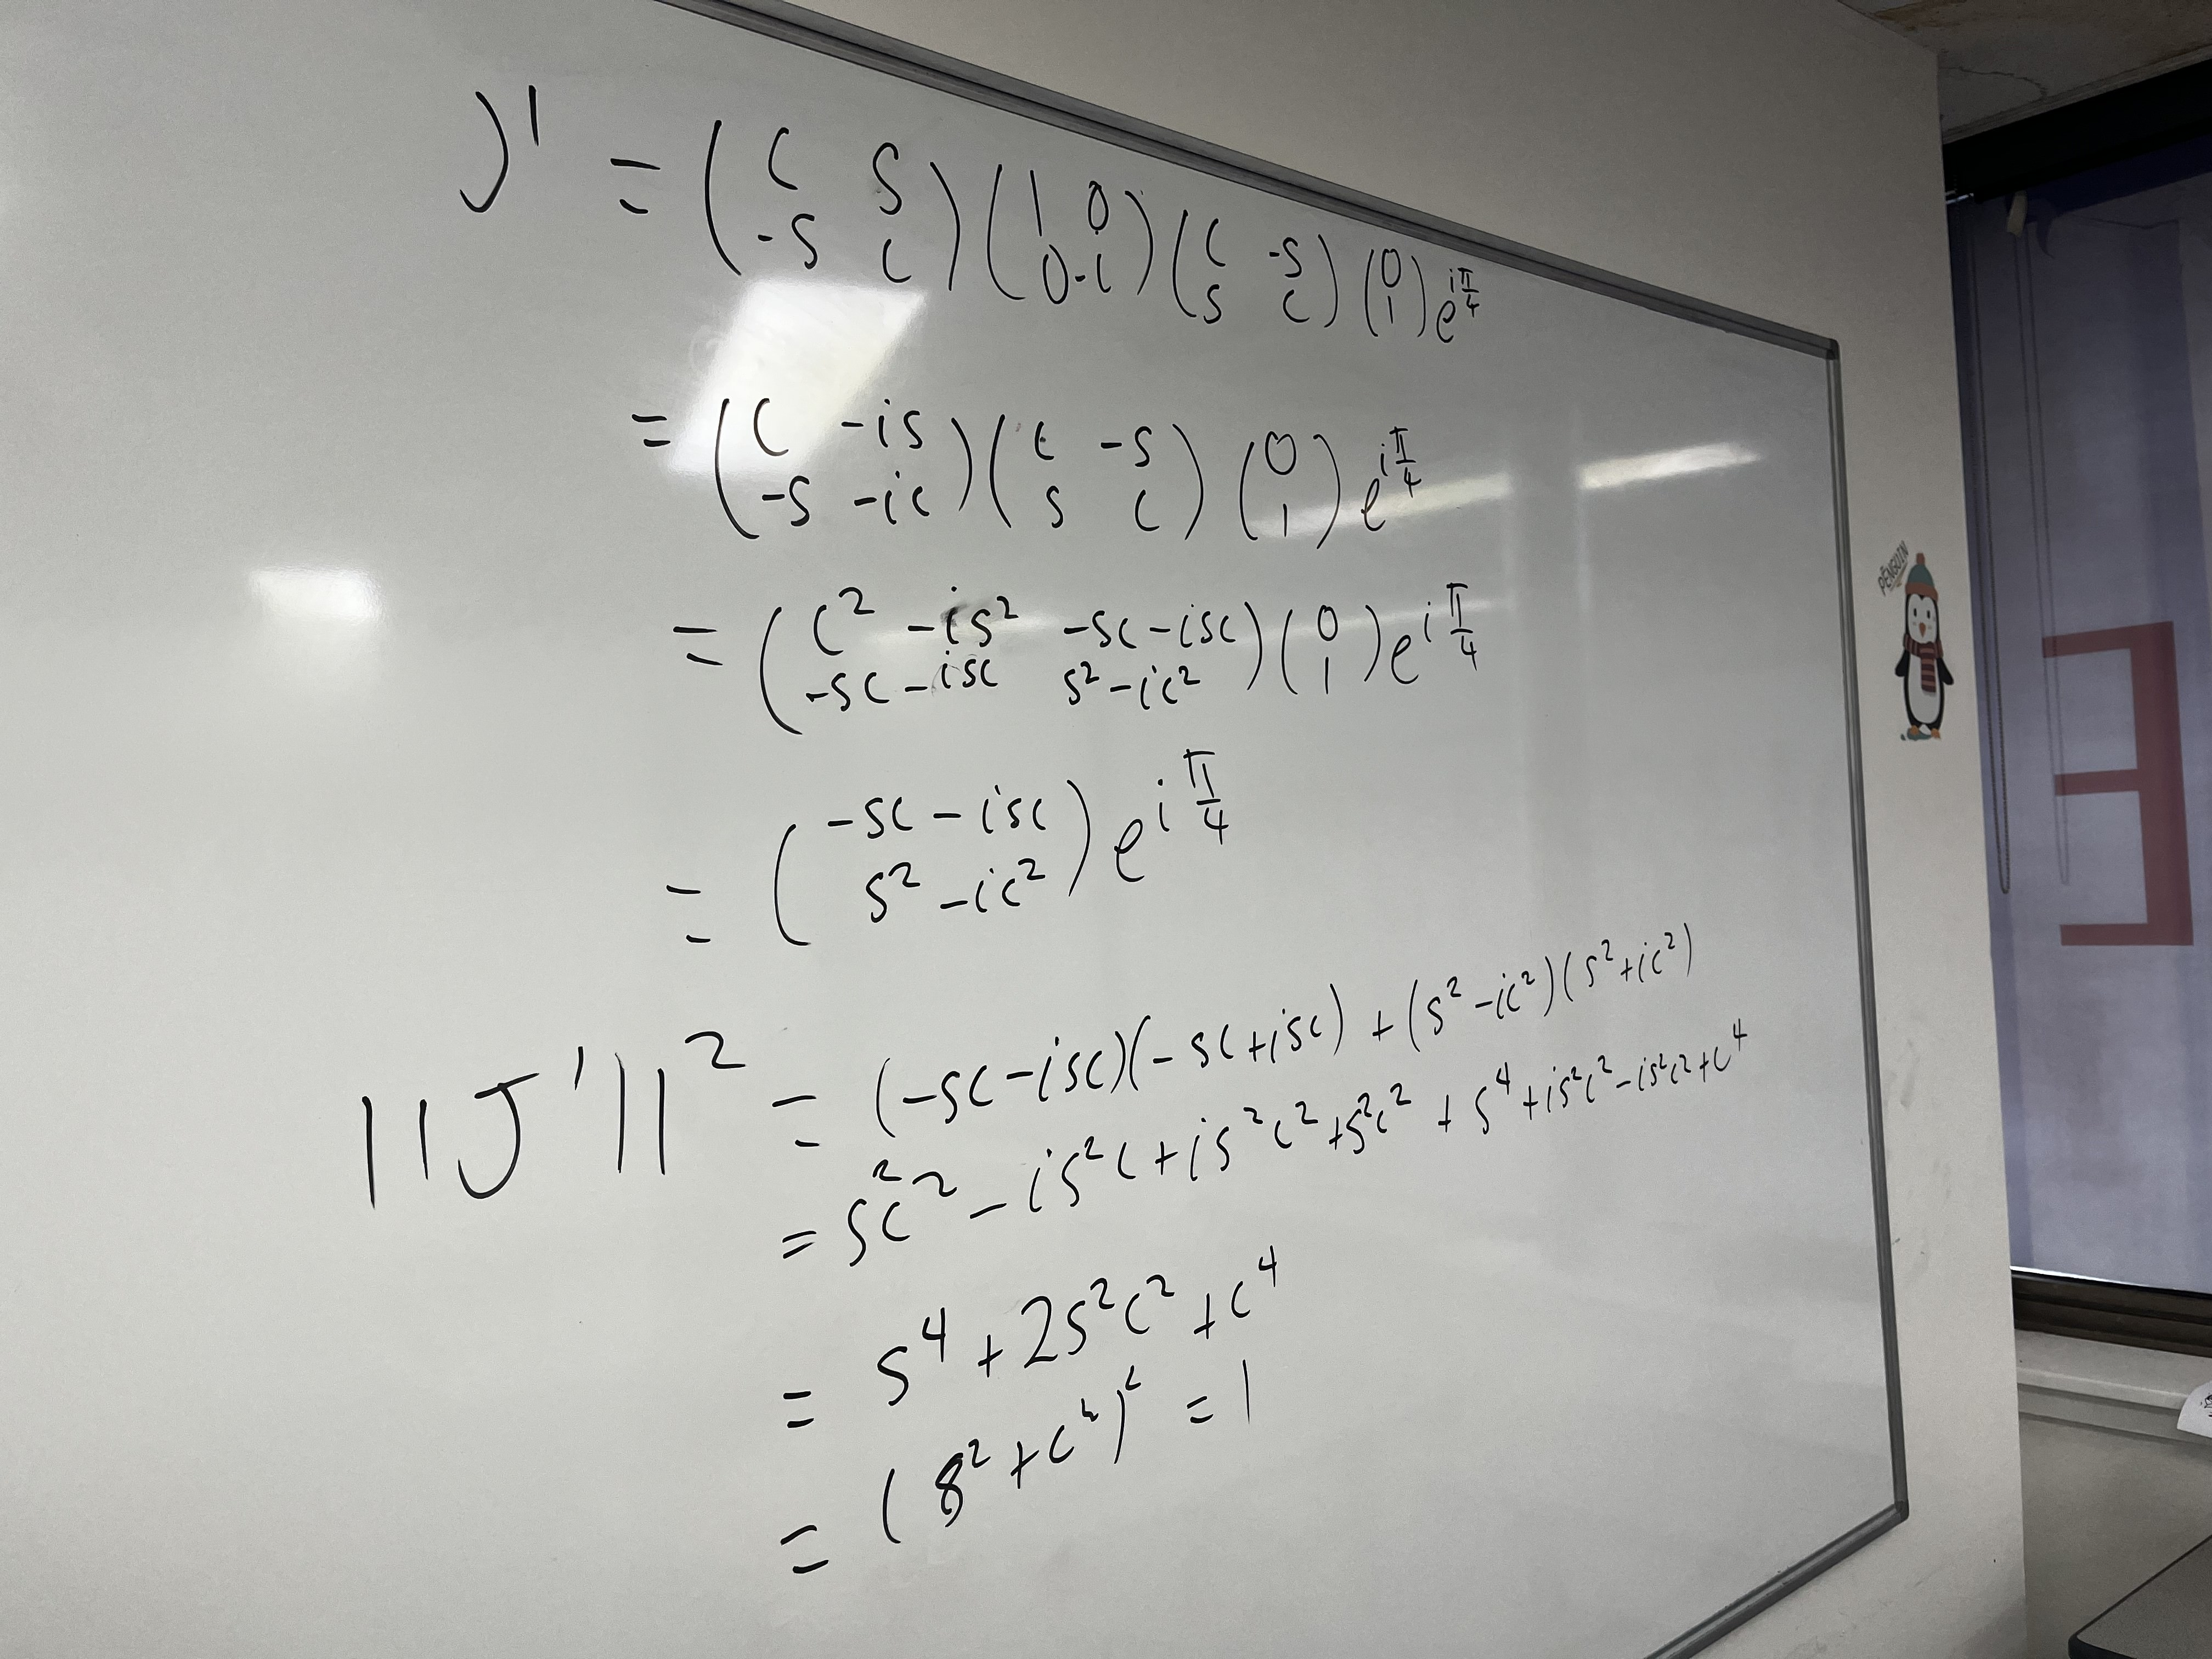
\includegraphics[width=0.8\textwidth]{circpol.jpg}
\end{figure}
\subsubsection{Reflectance coefficient using Jones matrices} \label{eq:derivation2}
\begin{figure}[H]
    \centering
    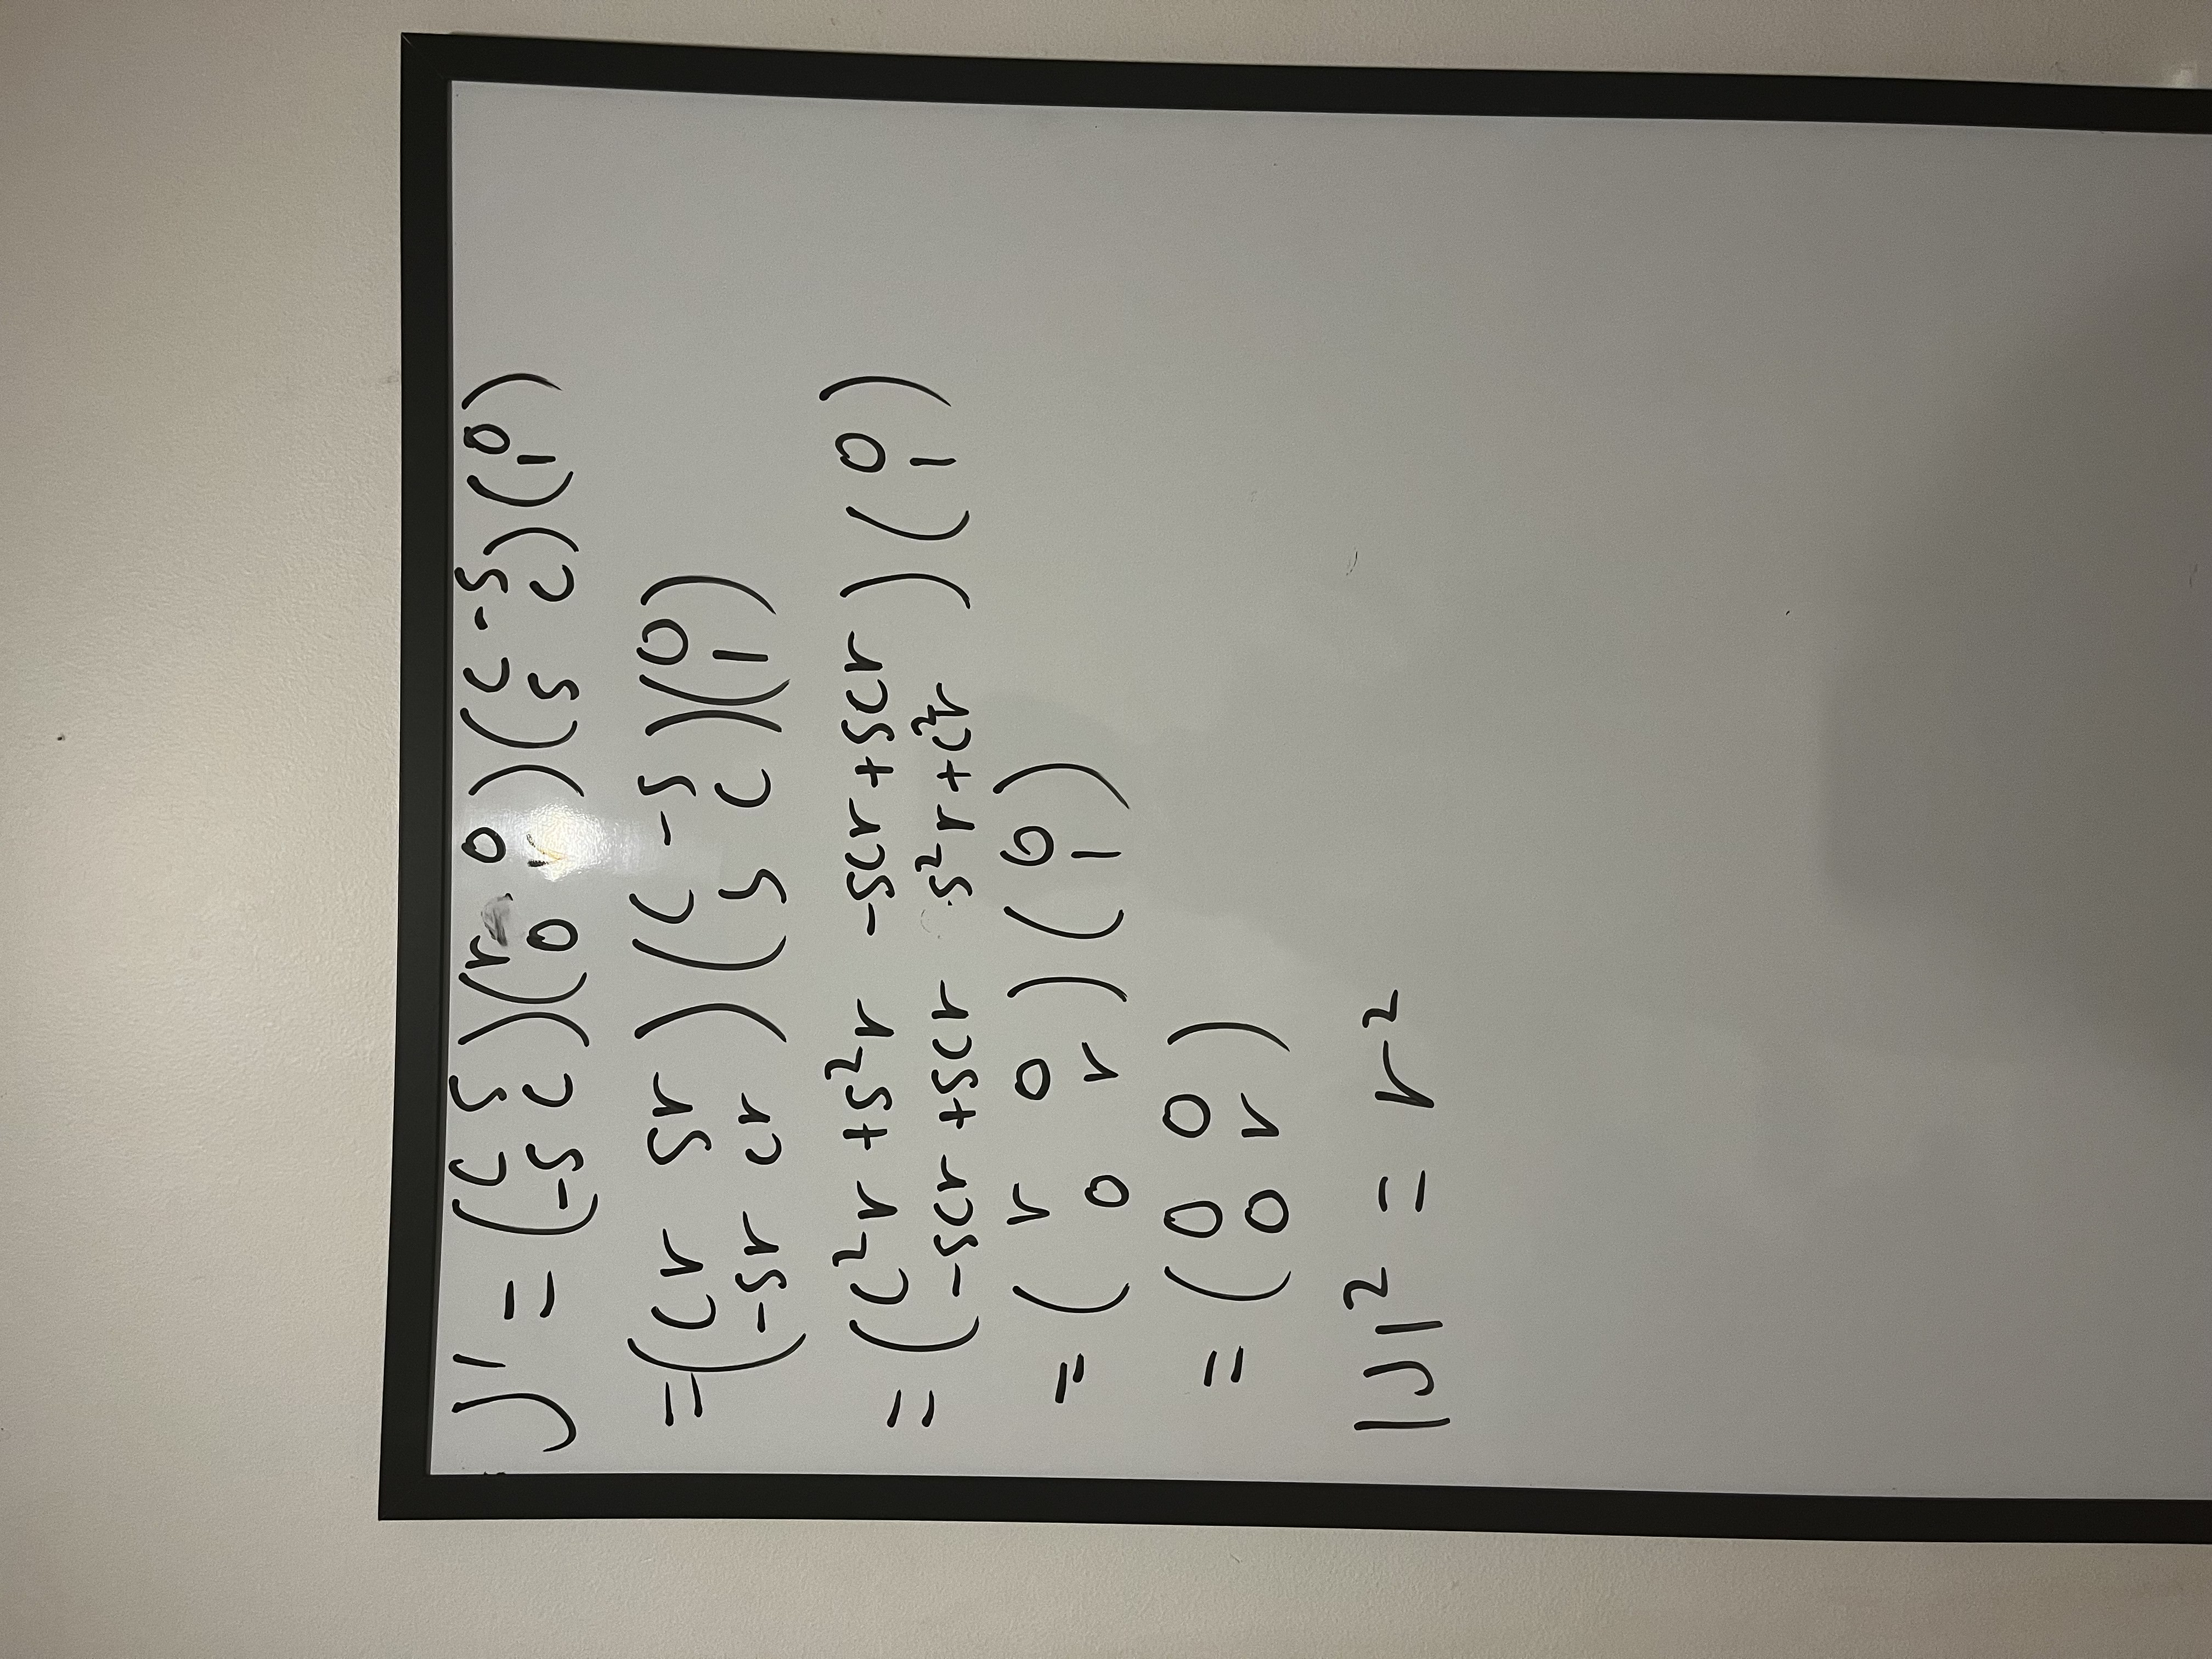
\includegraphics[width=1.2\textwidth,angle=270,origin=c]{reflectance.jpg}
\end{figure}

\subsection{Curve fitting}

Python was used to create theoretical models to best fit the 
experimental data. First the cosine squared function was defined 
with parameters: $I_0$, theta0 and offset with variable theta. The 
amplitude is given by the initial intensity, $I_0$, the phase shift 
is given by theta0 and the vertical displacement of the funtion 
is given by the parameter offset.

\begin{python}
def curve(theta,I_0,theta0,offset):
    return I_0 * np.cos(np.radians((theta - theta0)))**2 + offset
\end{python}

Using the scipy optimize package, the curve fit function can be 
used which uses a least-squares algorithm to guess the parameters 
that best fits the data input. An example can be seen below,

\begin{python}
x = data['Angle (degrees)']
y = data['Current (micro amps)']

param,covariance = sp.curve_fit(curve,x,y)
\end{python}

The return of the function is of course an array, param, of the best 
fitting parameters.

Rather than plotting the model as a function of the experimental data,
the model was plotted over a a higher resolution of x values to provide 
a smoother curve.

\begin{python}
x_smooth = np.linspace(x.min(),x.max(),1000)
y_smooth = curve(x_smooth,*param)
plt.plot(
    x_smooth,
    y_smooth,
    label=rf'$I_0$={param[0]:.2f}, $\theta_0$ = {param[1]:.2f}, offset = {param[2]:.3f}'
)
\end{python}

The Fresnel equations were also fitted using the following code.

\begin{python}
def fresnel_s(theta, E_p, I_0, n=1.5, epsilon=1e-4):
    theta_rad = np.radians(theta)
    
    small_angle_mask = np.abs(theta_rad) < epsilon
    large_angle_mask = ~small_angle_mask
    
    result = np.zeros_like(theta_rad)
    
    result[small_angle_mask] = I_0 + E_p * (theta_rad[small_angle_mask] ** 2) / 2
    
    refracted_theta = np.arcsin(np.sin(theta_rad[large_angle_mask]) / n)
    result[large_angle_mask] = (
        E_p * np.tan(theta_rad[large_angle_mask] - refracted_theta) / 
        np.tan(theta_rad[large_angle_mask] + refracted_theta) + I_0
    )
    
    return result

def fresnel_p(theta, E_p, I_0, n=1.5, epsilon=1e-4):
    theta_rad = np.radians(theta)
    
    small_angle_mask = np.abs(theta_rad) < epsilon
    large_angle_mask = ~small_angle_mask
    
    result = np.zeros_like(theta_rad)
    
    result[small_angle_mask] = I_0 + E_p * (theta_rad[small_angle_mask] ** 2) / 2
    
    refracted_theta = np.arcsin(np.sin(theta_rad[large_angle_mask]) / n)
    result[large_angle_mask] = (
        E_p * np.tan(theta_rad[large_angle_mask] - refracted_theta) / 
        np.tan(theta_rad[large_angle_mask] + refracted_theta) + I_0
    )
    
    return result
\end{python}

\subsection{Solving simutaneous equations} \label{eq:solved}
\begin{python}
# Define the functions for fsolve
def equations(vars):
    x, y = vars
    eq1 = np.arctan(2 * x / (1 - x**2 - y**2)) - 0.216
    eq2 = ((1 - x)**2 + y**2) / ((1 + x)**2 + y**2) - 0.65
    return [eq1, eq2]

# Provide an initial guess for (x, y)
initial_guess = (0.5, 0.5)
solution = fsolve(equations, initial_guess)
print(solution)
\end{python}

\end{document}